%!TEX root = ../memoire.tex

\chapter{GenDR: un réalisateur profond générique}\label{chapgendr}

GenDR (pour \emph{Generic Deep Realizer}) est un réalisateur profond multilingue \citep{lareau18} qui a hérité de l'architecture de MARQUIS \citep{WannerMARQUISGENERATIONUSERTAILORED2010} (section\ref{sectionmarquis}). Comme son prédécesseur, GenDR est un transducteur de graphes basé sur la \ac{TST}, et ses dictionnaires et grammaires fonctionnent essentiellement de la même manière.

Cependant, contrairement à MARQUIS, GenDR génère uniquement des structures syntaxiques de surface, car ce réalisateur se concentre sur la modélisation de phénomènes langagiers profonds comme la lexicalisation et l'arborisation. Pour compléter la réalisation jusqu'au texte, il faudrait utiliser un réalisateur de surface qui prenne les outputs de GenDR en entrée et réalise du texte fléchi et linéarisé. À ce sujet, \cite{MilleSharedTaskProposal2017a} proposent une compétition pour créer un réalisateur de surface multilingue capable de prendre en input des arbres de dépendances universels \citep{NIVRE16.348}. On pourrait alors envisager de mapper l'output de GenDR sur ce type de structure.

En tant qu'héritier de MARQUIS, GenDR en reprend les composantes de base pour modéliser les phénomènes langagiers élémentaires comme la lexicalisation simple, la complémentation et la modification. Ces règles forment le noyau du système et sont généralement partagées par l'ensemble des langues, tandis que les phénomènes grammaticaux spécifiques comme l'insertion des auxilaires ou des déterminants sont régis par des règles propres à chaque langue.

%%%%%%%%%%%%%%%%%%%%%%%%%%%%%%%%%%%%%%%%%%%%%%%%%%%%%%%
% --------- A R C H I T E C T U R E  GENDR  ---
%%%%%%%%%%%%%%%%%%%%%%%%%%%%%%%%%%%%%%%%%%%%%%%%%%%%%%%
\section{Architecture de GenDR}

Les composantes lexicales et grammaticales de GenDR sont prises en charge par le transducteur de graphes MATE \citep{BohnetDevelopmentEnvironmentMTTbased2000a,BOHNET10}. Ainsi, pour mieux comprendre comment la réalisation se déroule dans GenDR, il faut d'abord présenter les composantes de ce logiciel.

MATE a été conçu à la base pour implémenter la \ac{TST} dans le but de générer du texte. Tous les niveaux de représentation (voir section \ref{sec:semsynt}) de la \ac{TST} correspondent à des graphes et la transformation d'un graphe en un autre est assurée par des ensembles de règles modélisant chaque interface (module sémantique et module syntaxique). En plus d'opérer la transduction de graphes, MATE a aussi été conçu pour tester, développer et maintenir une grammaire computationnelle, ce qui nous permet de réaliser du texte tout en testant les fondements théoriques de la \ac{TST}.

MATE comprend un éditeur de dictionnaires, de graphes et de grammaires. Les dictionnaires encodent les propriétés des unités sémantiques et lexicales, alors que les grammaires sont composées de règles modélisant le passage d'un niveau de représentation à un autre. L'éditeur de graphes permet de construire et de visualiser ceux-ci. MATE comprend aussi un module d'inspection permettant de voir le déroulement de l'application des règles. Cet outil s'avère très utile au développement d'une grammaire, puisqu'il permet de cerner à quel endroit la réalisation a échoué. Pour plus de détails, voir \cite{BohnetOpensourcegraph2010,LambreyImplementationcollocationspour2017,LambreyGECOv1User2016}.

%%%%%%%%%%%%%%%%%%%%%%%%%%%%%%%%%%%%%%%%%%%%%%%%%%%%%%%
% ---------D I C T I O N N A I R E  ------------------
%%%%%%%%%%%%%%%%%%%%%%%%%%%%%%%%%%%%%%%%%%%%%%%%%%%%%%%

\subsubsection{Dictionnaires}\label{sec:dictio}

GenDR utilise trois dictionnaires pour décrire le vocabulaire qui sera utilisé dans les textes: un qui fait le pont entre les unités sémantiques et les unités lexicales, un qui décrit le comportement syntaxique des unités lexicales, et un qui décrit les fonctions lexicales. Nous excluerons le troisième dictionnaire de la discussion parce que nous ne traitons pas des fonctions lexicales dans ce mémoire.

\textbf{Le dictionnaire sémantique}, qu'on appelle \emph{semanticon}, est utilisé par le système lors du passage de la \ac{RSem} à la \ac{RSyntP}. Cette ressource décrit les lexicalisations possibles pour un sémantème donné. C'est une source importante de paraphrasage puisqu'une unité sémantique peut souvent se réaliser de plus d'une manière. Par exemple, en anglais, le sens \sem{owe} peut se réaliser par les lexèmes \lex{owe} (un verbe) et \lex{debt} (un nom).

\begin{figure}
  \caption{Échantillon du \emph{semanticon}}
	\label{fig:semanticon}
\begin{lstlisting}[language=mate]
owe { lex = owe
      lex = debt }
\end{lstlisting}
\end{figure}

\textbf{Le dictionnaire lexical}, appelé \emph{lexicon}, contient de l'information détaillée à propos des lexies d'une langue donnée. Les entrées contiennent: la \ac{DPOS}, la \ac{SPOS}, la diathèse et les \acp{GP}. Ces deux derniers concepts seront clarifiés à la fin du chapitre, section~\ref{sec:gp}, mais en résumé, la diathèse d'une lexie assure la correspondance entre ses actants sémantiques et ses actants syntaxiques, puis un \ac{GP} correspond à la description d'une construction syntaxique sélectionnée par un lexème.

Dans le \emph{lexicon}, ces propriétés (\ac{DPOS}, \ac{SPOS}, \ac{GP} et diathèse) ne sont pas toujours explicitées pour chaque entrée lexicale, puisque GenDR renferme un mécanisme d'héritage permettant de transmettre des traits entre lexèmes. Par exemple, à la figure~\ref{fig:lexicon}, le verbe \lex{owe} contient très peu d'information syntaxique parce qu'il hérite de plusieurs propriétés de la classe absraite \texttt{verb\_dit}, qui correspond à la classe des verbes ditransitifs. Cela permet à \lex{owe} d'hériter d'une partie du \ac{GP} de la classe ditransititive qui le domine. À son tour, la classe \emph{verb\_dit} hérite des traits de sa classe mère, \lstinline|verb_dit : verb_dt|. Autrement dit, la classe des verbes ditransitifs imbriquent les propriétés de la classe transitive, en plus de préciser la sélection d'un actant syntaxique de plus. Ainsi, le mécanisme d'héritage facilite grandement l'encodage des unités lexicales, car on n'a qu'à associer chaque nouvelle entrée lexicale à la classe abstraite qui lui correspond. Il en existe pour chaque partie du discours (verbes, noms, adjectifs, adverbes, prépositions, etc.).

On peut aussi bloquer l'héritage de traits pour une entrée lexicale donnée. Par exemple, la figure~\ref{fig:lexicon} illustre que la lexie \lex{owe} permet deux \ac{DPOS} différentes pour le deuxième actant syntaxique qu'elle contrôle: \lstinline!gp={II={dpos=Num}}! et \lstinline!gp={II={dpos=N}}!. Elle permet ainsi la sélection d'un actant de type nominal ou numéral, ce qui ne fait pas partie du régime de la classe abstraite \texttt{verb\_dit}.

\begin{figure}
  \caption{Échantillon du \emph{lexicon}}
	\label{fig:lexicon}
\begin{lstlisting}[language=mate]
predicate {
  gp = { 1 = I
         2 = II
         3 = III
         4 = IV
         5 = V
         6 = VI }
}
verb : predicate {
  dpos = V
  spos = verb
  gp = {
     I = {
        dpos = N
        rel = subjective
     }
  }
}
verb_dt : verb {                   // direct transitive
  gp = {
     II = {
        dpos = N
        rel = dir_objective

     }
  }
}
verb_dit : verb_dt {              // direct ditransitive
  gp = {
     III = {
        dpos = N
        rel = indir_objective
        prep = to  

     }
  }
}
[...]
owe : verb_dit {
  gp = { II = { dpos=Num } }
  gp = { II = { dpos=N } }
}
\end{lstlisting}
\end{figure}

Finalement, les dictionnaires anglais et français de GenDR contiennent les 1\,500 lexèmes les plus courants de chaque langue. Pour leur part, les dictionnaires lituanien \citep{dubinskaite17} et persan contiennent respectivement $\sim$180 et $\sim$60 lexèmes, assez pour tester le système.

%%%%%%%%%%%%%%%%%%%%%%%%%%%%%%%%%%%%%%%%%%%%%%%%%%%%%%%
% ---------G R A M M A I R E  ------------------
%%%%%%%%%%%%%%%%%%%%%%%%%%%%%%%%%%%%%%%%%%%%%%%%%%%%%%%

\subsubsection{Grammaires}
La grammaire de GenDR est organisée autour de deux modules de règles: le module sémantique (\ac{RSem}--\ac{RSyntP}) et le module syntaxique (\ac{RSyntP}--\ac{RSyntS}).

Le module \ac{RSem}--\ac{RSyntP} s'occupe de faire l'arborisation (algorithme \emph{top-down}) et la lexicalisation profonde (sélection des lexèmes pour représenter les sémantèmes) de l'input. Ce module est divisé en trois groupes de règles: le c\oe{}ur partagé par toutes les langues, les fonctions lexicales, et les règles spécifiques à chaque langue. Le module sémantique contient 21 règles générales, dont la plupart sont héritées de MARQUIS, et 132 règles de lexicalisation, dont la plupart gèrent des patrons de collocations \citep{LambreyImplementationcollocationspour2017}.

Le module \ac{RSyntP}--\ac{RSyntS} s'occupe de l'arborisation et la lexicalisation de surface (ajout des mots fonctionnels et des relations de surface). Il est divisé en deux: les règles partagées par toutes les langues et les règles propres à chaque langue. Le module syntaxique en contient nettement moins: vingt règles, dont douze partagées entre les langues. Nous construirons donc la nouvelle version de GenDR à partir des bases mises en place par \cite{LambreyImplementationcollocationspour2017}, \cite{dubinskaite17} et \cite{lareau18}. Toutefois, nous avons retiré les patrons de collocation de notre système pour mieux nous concentrer sur le régime des verbes sans nous perdre dans des interactions inutilement complexes entre les modules.

Nous présenterons en détail les règles principales de ces deux modules dans les sections \ref{sec:arbo} et \ref{sec:exemple}. 

Pour donner une meilleure idée de l'allure de l'éditeur de règles, la figure~\ref{fig:root} présente une règle du module sémantique-syntaxe profonde. Toutes les règles sont décrites dans ce format. D'abord, en haut, nous avons l'interface dans laquelle la règle opère, suivi du nom de la règle et de l'identification de son groupe. Dans la partie gauche (\emph{Leftside}) on retrouve les n\oe{}uds et arcs du graphes de départ, puis dans la partie droite (\emph{Rightside}) on retrouve le graphe créé en sortie. Finalement, la partie du bas contient les conditions d'application de la règle donnée. Nous verrons en détails l'application concrète de la règle~\ref{fig:root} à la section~\ref{sec:arbo}. Pour une présentation plus détaillé de la création de règles, voir le manuel de GÉCO \citep{LambreyGECOv1User2016}.

\begin{figure}[htb]
	\centering
	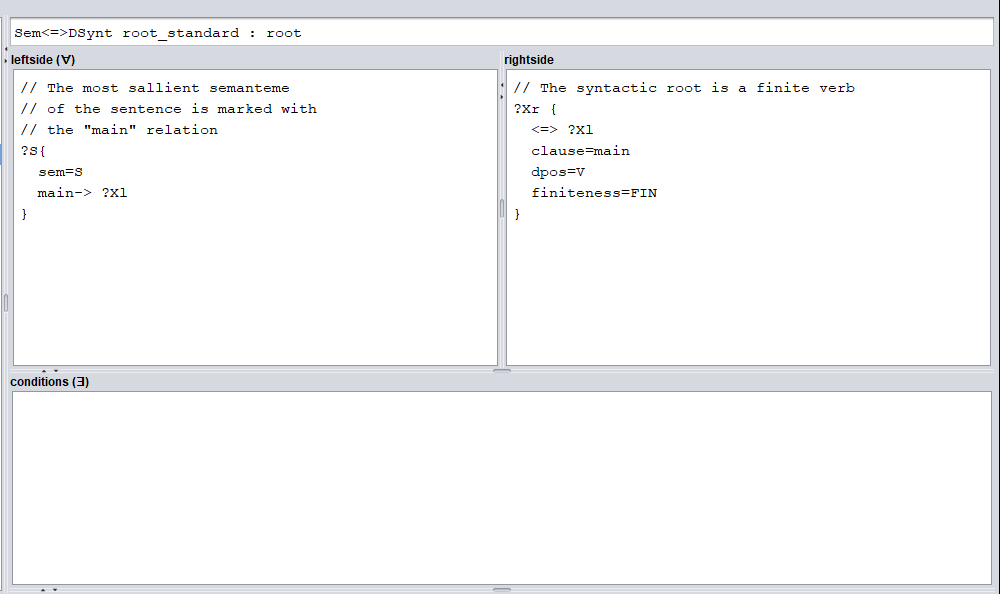
\includegraphics[width=1\textwidth, trim = {0cm 0cm 0cm 0cm},clip]{ch3/figs/grammaire.png}
	\caption{Règle créant la racine syntaxique}
	\label{fig:root}
\end{figure}

%%%%%%%%%%%%%%%%%%%%%%%%%%%%%%%%%%%%%%%%%%%%%%%%
% ---------G R A P H E S ------------------
%%%%%%%%%%%%%%%%%%%%%%%%%%%%%%%%%%%%%%%%%%%%%%%%

\subsubsection{Graphes}\label{entree-sortie}

Maitenant que nous avons fait un survol des dictionnaires et de la grammaire, il ne nous reste qu'à présenter les graphes. Dans un premier temps nous présenterons brièvement la construction d'un graphe d'input, puis nous montrerons à quoi ressemblent les graphes en output.

L'input du réalisateur GenDR est un graphe sémantique \citep{mel2012semantics} où les prédicats sont liés à leurs arguments par des relations numérotées qui indiquent la position logique de l'argument. La figure~\ref{fig:debt} montre comment on construit un graphe sémantique dans MATE.

\begin{figure}
  \caption{Graphe sémantique en mode textuel}
	\label{fig:debt}
\begin{lstlisting}[language=mate]
structure Sem debt {
  S {
    owe {
    tense=PRES
    1-> Paul {class=proper_noun}
    2-> "\$500K" {class=amount}
    3-> bank {number=SG definiteness=DEF}}
    main-> owe } }
\end{lstlisting}
\end{figure}

Toutefois, MATE offre aussi une version graphique pour encoder et visualiser les graphes (voir la figure~\ref{fig:graphesem}).

\begin{figure}[htb]
	\centering
	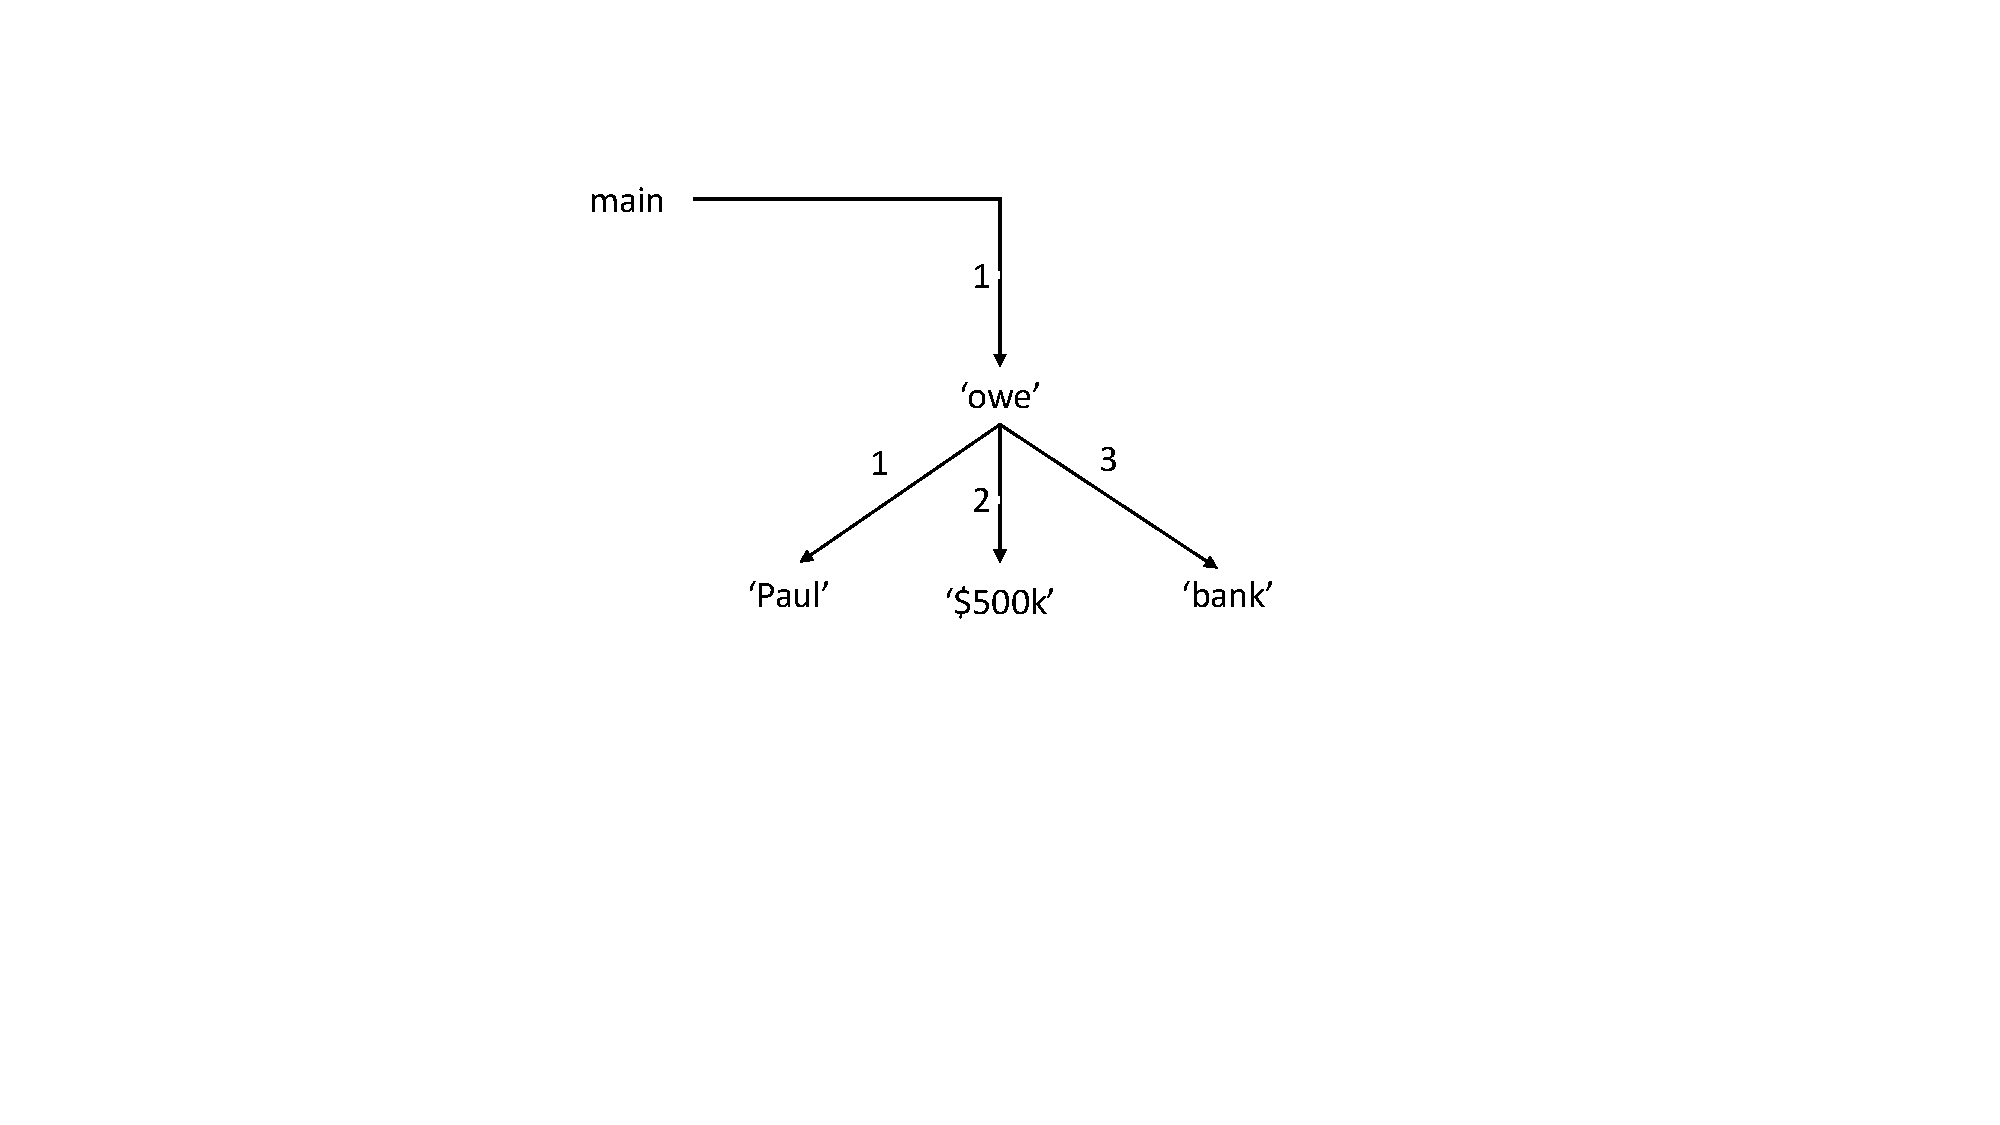
\includegraphics[width=1\textwidth, trim = {0cm 7cm 0cm 3cm},clip]{ch3/figs/owe_sem.pdf}
	\caption{Graphe sémantique en mode visuel}
	\label{fig:graphesem}
\end{figure}

L'éditeur de graphes de MATE nous permet de construire les structures sémantiques d'input et de visualiser les graphes en output. Pour l'input donné au listing~\ref{fig:debt} , GenDR réalise six structures syntaxiques de surface. Celles-ci peuvent être visualisées dans MATE grâce au module de graphes. La figure~\ref{fig:realsurfex} est un exemple d'output visuel qu'offre GenDR et la figure~\ref{fig:6realsurf} montre à quoi ressembleraient les six représentations possibles si on les linéarisait. Cette variété de représentations est possible grâce au mécanisme de paraphrasage de GenDR.

\begin{figure}[htb]
	\centering
	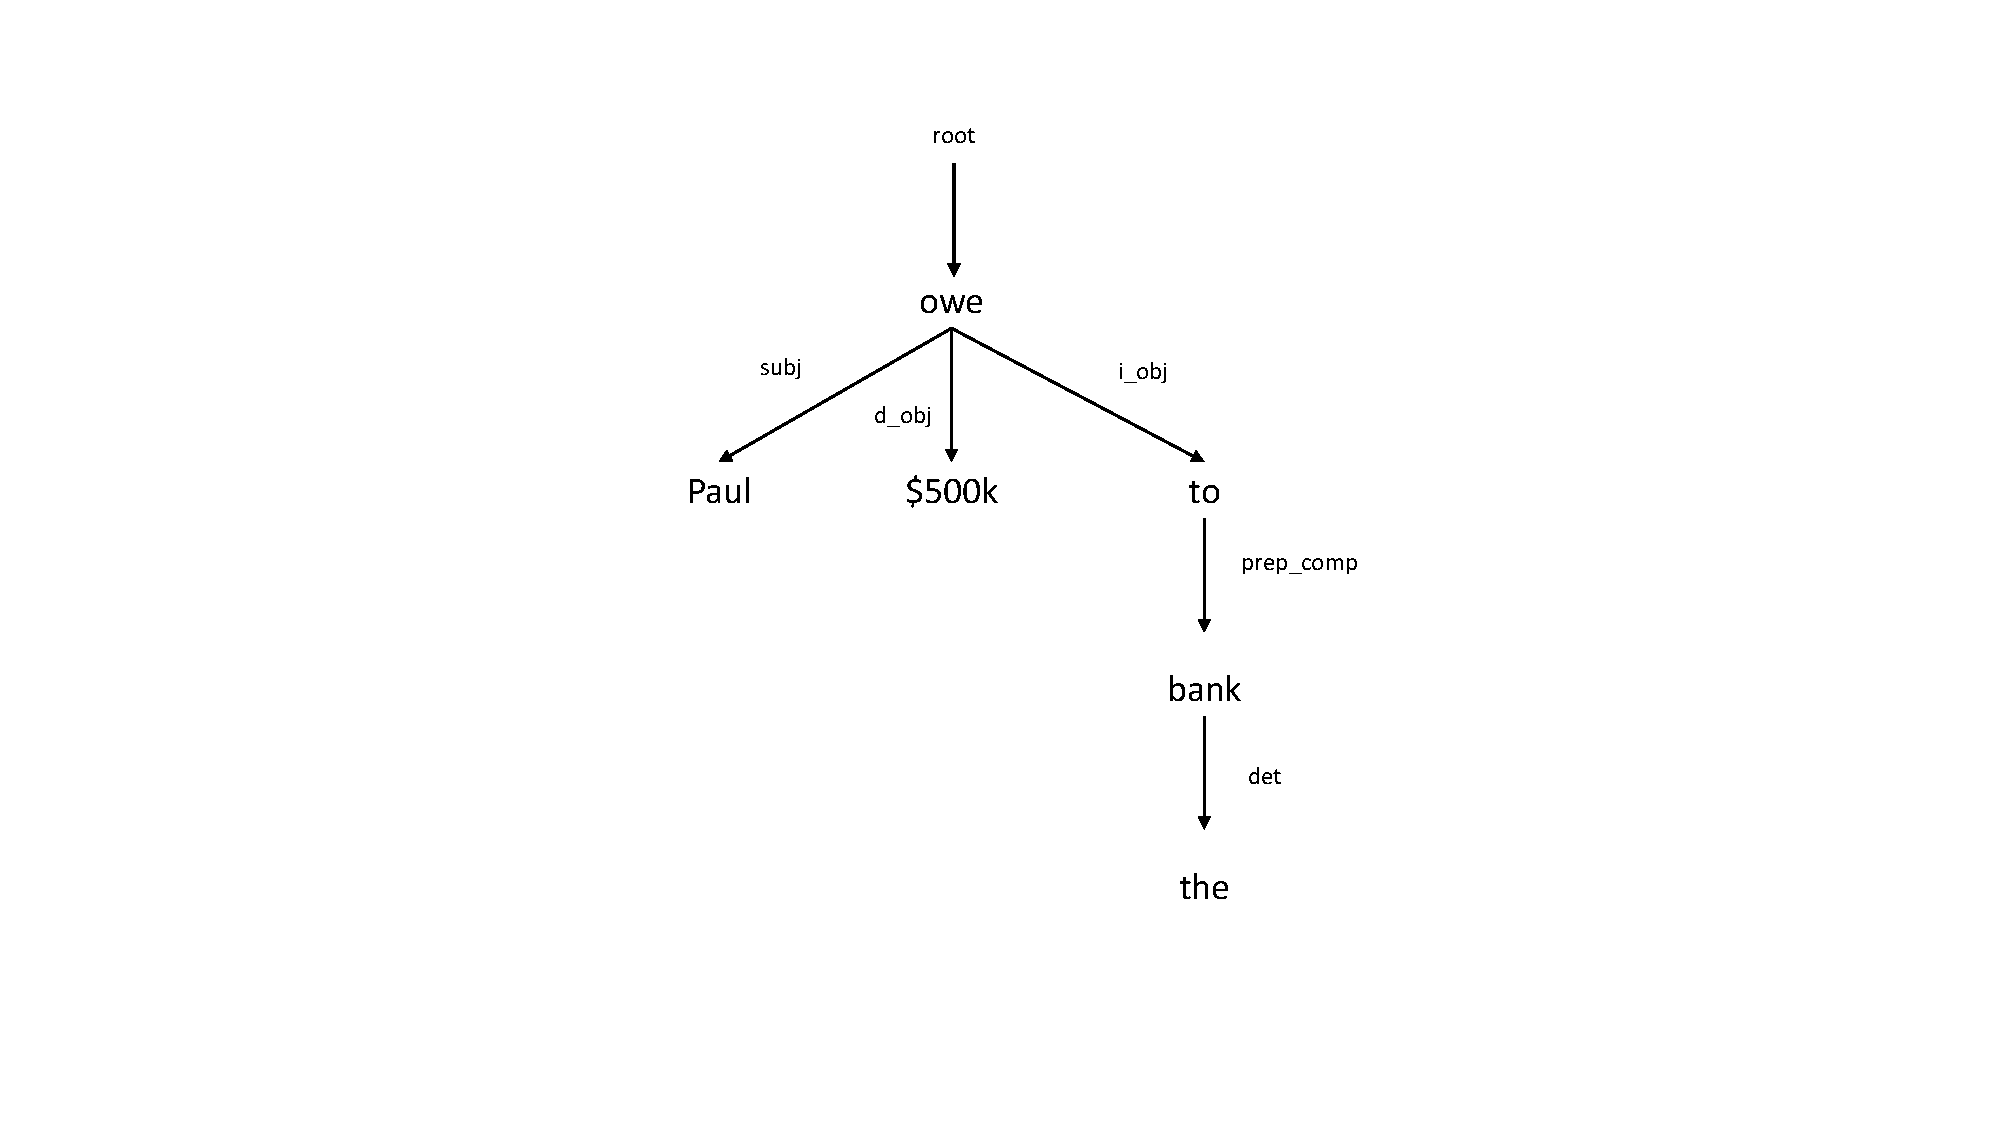
\includegraphics[width=1\textwidth, trim = {0cm 3cm 3cm 2cm},clip]{ch3/figs/realsurfex.pdf}
	\caption{Réalisation de surface}
	\label{fig:realsurfex}
\end{figure} 

\begin{figure}[htb]
	\centering
	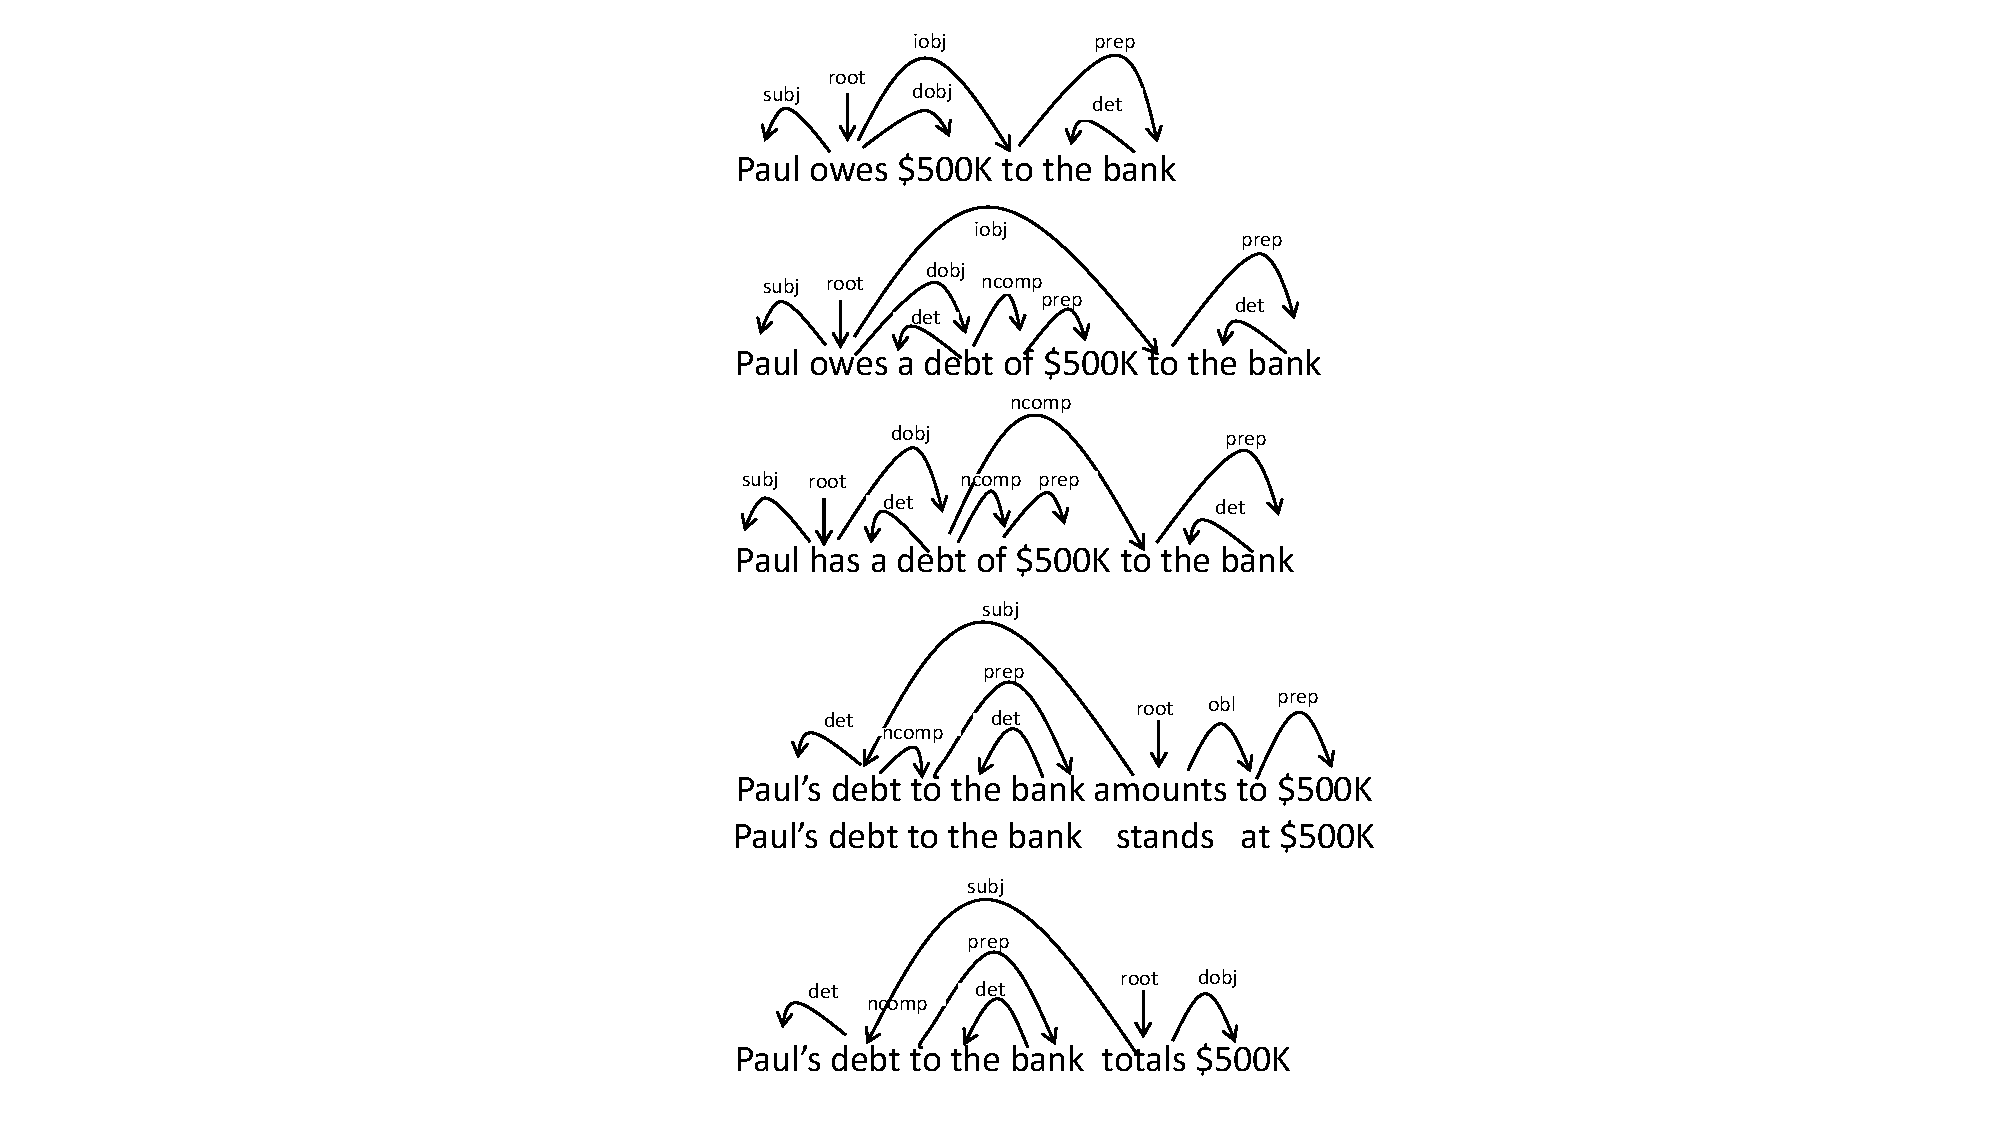
\includegraphics[width=1.3\textwidth, trim = {6cm 0cm 0cm 0cm},clip]{ch3/figs/6_real_surface.pdf}
	\caption{Six réalisations syntaxiques de surface \citep{lareau18}}
	\label{fig:6realsurf}
\end{figure}

Pour obtenir une réalisation linéarisée et fléchie, il nous faudrait utiliser un réalisateur de surface. Pour cela, on peut envisager d'interfacer la sortie de GenDR avec divers réalisateurs de surface \citep{DaoustJSREALTextRealizer2015, DBLP:conf/enlg/MolinsL15, GattSimpleNLGRealisationEngine2009, BelzFirstSurfaceRealisation2011}.

%%%%%%%%%%%%%%%%%%%%%%%%%%%%%%%%%%%%%%%%%%%%%%%%%%%%%%%%%%%%%%%%%%%%%%%%%%%%%
% --------- I N T E R F A C E   S É M A N T I Q U E- S Y N T A X E ---------
%%%%%%%%%%%%%%%%%%%%%%%%%%%%%%%%%%%%%%%%%%%%%%%%%%%%%%%%%%%%%%%%%%%%%%%%%%%%%

\section{Interface sémantique-syntaxe en TST}\label{sec:semsynt}

Dans cette section, nous décrirons l'interface sémantique-syntaxe dans le cadre de la \ac{TST} afin de mieux rendre compte des deux processus nécessaires au passage de la sémantique à la syntaxe: l'arborisation et la lexicalisation. Ces opérations sont la force de GenDR en termes de paraphrasage et de la flexibilité du système à réaliser des phénomènes langagiers profonds. Pour mieux comprendre où se situent ces procédés dans la modélisation du langage, nous ferons un très bref retour sur les fondements de ce cadre théorique.

La \ac{TST} vise la modélisation formelle de la correspondance entre les \emph{Sens} et les \emph{Textes} \citep{DBLP:conf/coling/JolkovskyM67, MelcukVerslinguistiqueSensTexte1997, PolgueretheorieSensTexte1998}. La figure~\ref{fig:modeletst} (qui est empruntée à \cite{PolgueretheorieSensTexte1998}) présente comment fonctionnent ces modèles qui sont des machines virtuelles prenant en entrée des représentations sémantiques d'énoncés pour générer du texte.

\begin{figure}[htb]
	\centering
	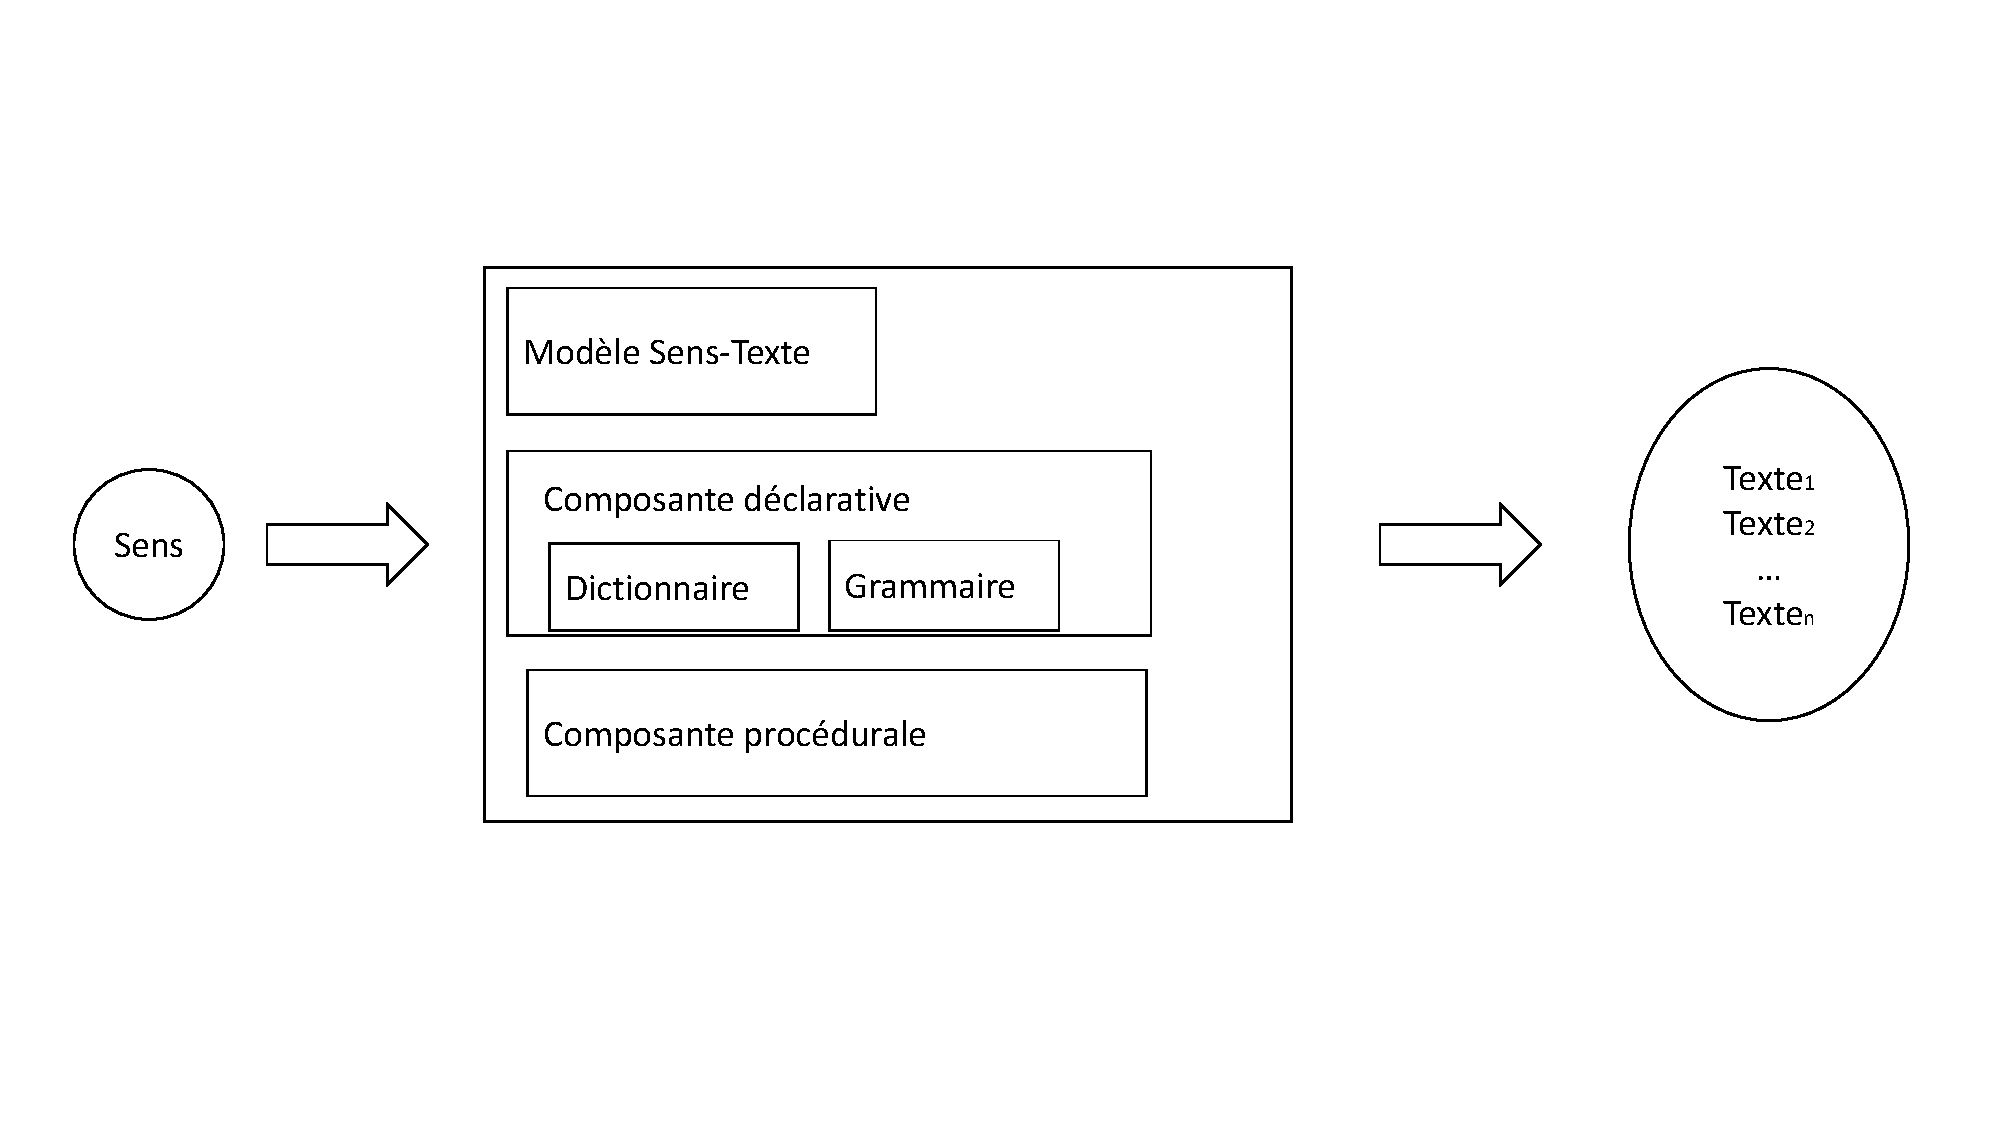
\includegraphics[width=1\textwidth, trim = {0cm 4cm 0cm 4cm},clip]{ch3/figs/polguere1.pdf}
	\caption{Structure d'un modèle Sens-Texte \citep{PolgueretheorieSensTexte1998}}
	\label{fig:modeletst}
\end{figure}

Pour se rendre au \emph{Texte} final, le \emph{Sens} traverse de nombreux niveaux de représentation. La figure~\ref{fig:processustst} illustre les transformations que l'input doit subir succesivement et, parallèlement, le formalisme utilisé pour représenter les niveaux.

\begin{figure}[htb]
	\centering
	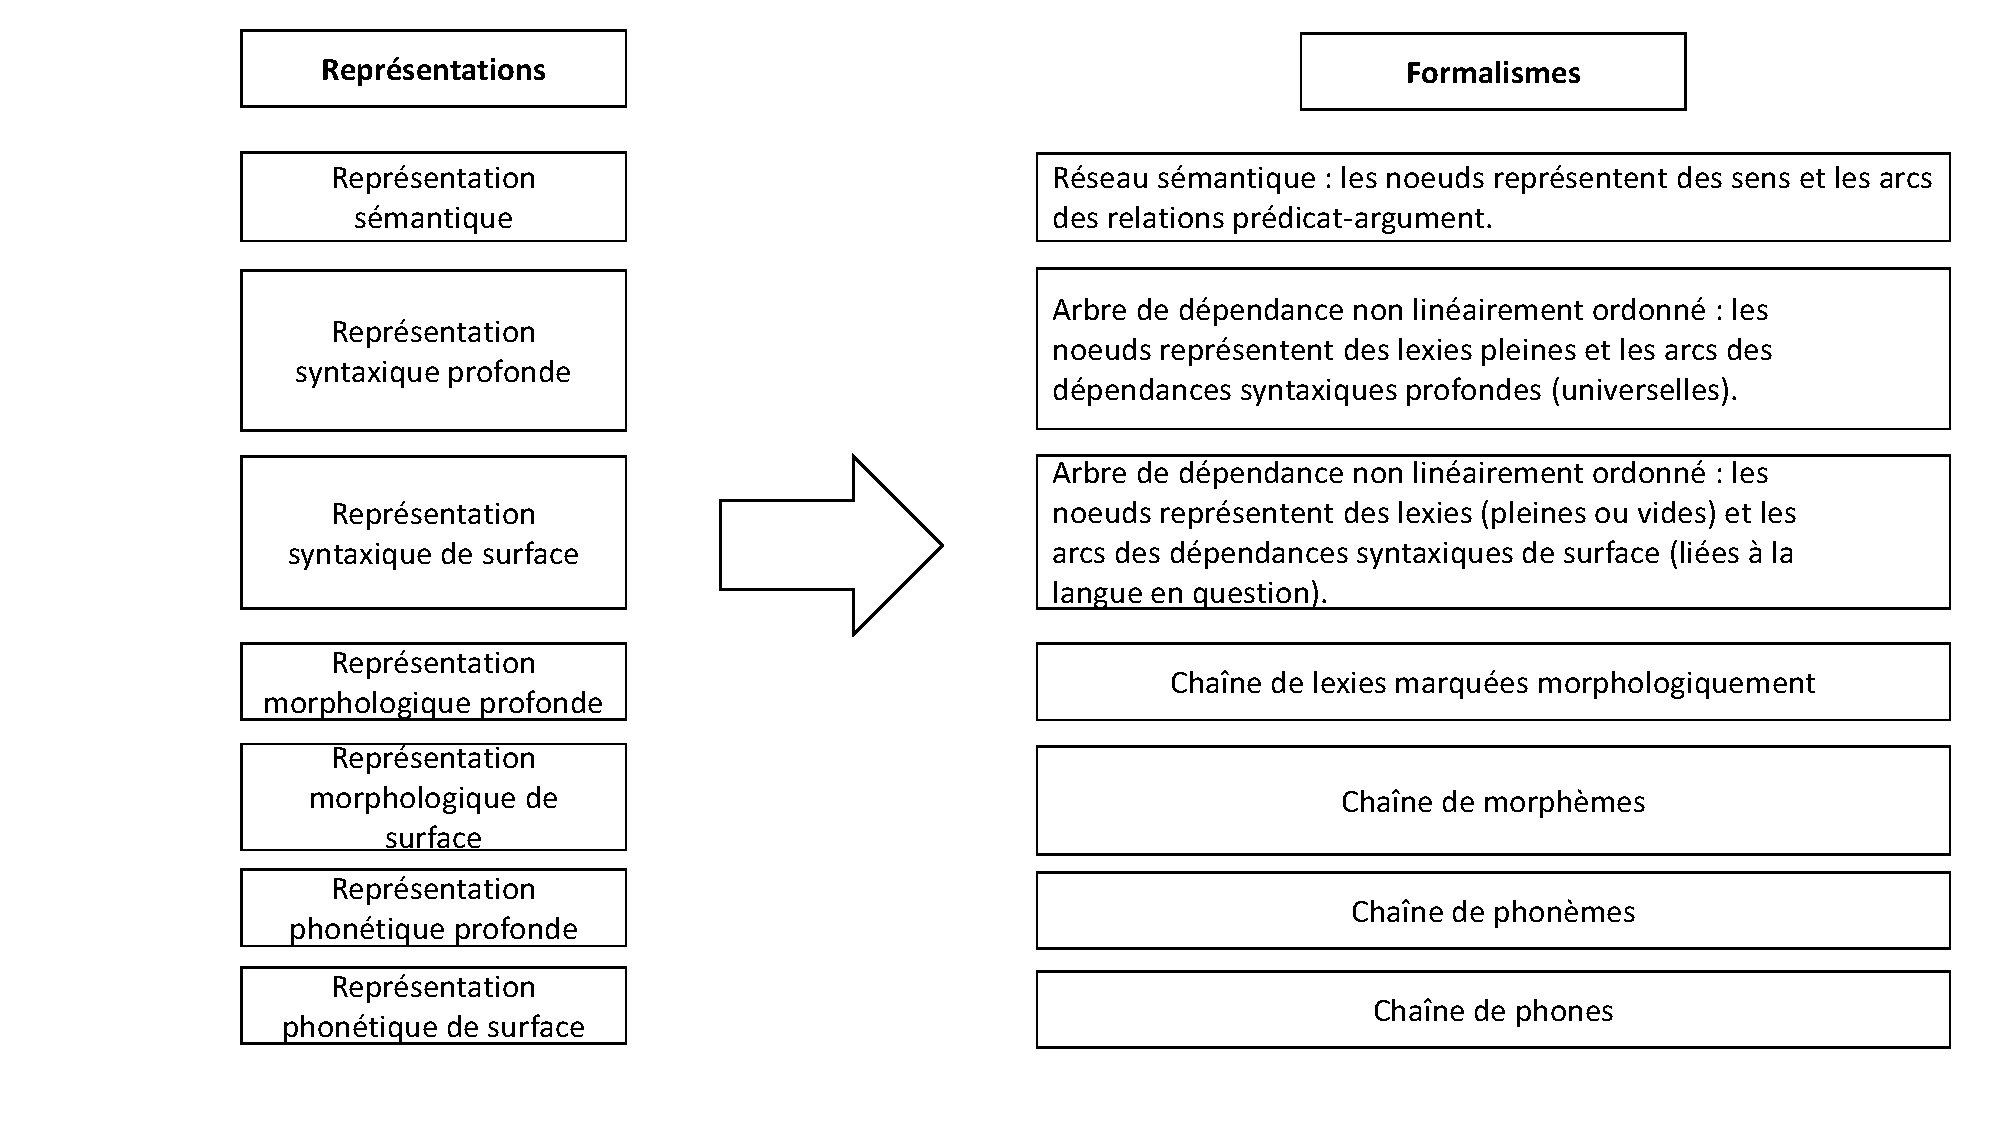
\includegraphics[width=1\textwidth, trim = {0cm 0cm 0cm 0cm},clip]{ch3/figs/polguere2.pdf}
	\caption{Processus d'un modèle Sens-Texte \citep{PolgueretheorieSensTexte1998}}
	\label{fig:processustst}
\end{figure}

%%%%%%%%%%%%%%%%%%%%%%%%%%%%%%%%%%%%%%%%%%%%
% --------- A R B O R I S A T I O N  ------
%%%%%%%%%%%%%%%%%%%%%%%%%%%%%%%%%%%%%%%%%%%

\subsection{Arborisation}\label{sec:arbo}

L'arborisation est le processus de transformation d'un graphe sémantique acyclique (DAG) en arbre de dépendance. Nous la décrirons à la fois d'un point de vue théorique et d'un point de vue appliqué.

Selon la \ac{TST}, la structure syntaxique d'un énoncé correspond à l'ensemble des liens de dependances fonctionnelles qui existent entre les unités lexicales de cet énoncé \citep{melcuk1988}. Cette approche syntaxique provient de \cite{TesniereElementssyntaxestructurale1965} qui est le premier à l'avoir théorisée. Formellement, le passage de la \ac{RSem} à la \ac{RSyntP} se fait grâce à la combinaison de l'arborisation et la lexicalisation. L'arborisation se fait ainsi à partir d'une structure sémantique qui subit des transformations grâces à l'application de règles de correspondances sémantiques pour qu'il en résulte un arbre de dépendances profond. Pour illustrer ce qu'est l'arborisation, nous reprendrons la description de \cite{lareau18} dans le contexte de GenDR. L'arbre syntaxique profond est construit avec un algorithme \emph{top-down} qui est emprunté de MARQUIS, mais qui est, à la base, inspiré de \cite{PolguereStructurationmisejeu1990}. Nous l'avions brièvement illustré avec la figure \ref{fig:marquis} lorsque nous avions présenté MARQUIS et FORGe.

Dans GenDR, l'arborisation s'opère en trois étapes \citep{lareau18}:

\begin{enumerate}
  \item \textbf{Création de la racine}.
  La première règle appliquée s'appelle \emph{root\_standard}, elle construit la racine de l'arbre syntaxique à partir du \ac{ND} de la structure sémantique. À cette étape, la racine n'est pas étiquetée par un lexème encore, donc le n\oe{}ud est vide. Toutefois, ce n\oe{}ud se fait généralement imposer les contraintes suivantes dans les langues européennes: on exige que ce soit un verbe et qu'il soit fini, puisque ce sont généralement les verbes qui contrôlent la structure d'un énoncé. Bref, la détermination de la racine correspond au processus de hiérarchisation de \cite{PolguereStructurationmisejeu1990} puisqu'on détermine le n\oe{}ud qui dominera tous les autres.

  \item \textbf{Lexicalisation de la racine}.
  Une fois que la racine a été créée et contrainte, on applique une règle de lexicalisation (appellée \emph{lex\_standard}) qui permet au système de fouiller dans les dictionnaires pour trouver un lexème qui correspondra au sens demandé tout en respectant les contraintes imposées. Ainsi, il faut que le lexème sélectionné corresponde au \ac{ND} en sémantique et qu'il respecte les contraintes sur le n\oe{}ud.

  \item \textbf{Application des règles actancielles}.
  Une fois que le n\oe{}ud racine est lexicalisé, GenDR récupère les informations encodées dans le patron de régime de la racine pour savoir comment effectuer le passage des arcs sémantiques aux arcs syntaxiques (la diathèse). Autrement dit, cette étape crée les arcs dépendant de la racine qui correspondent aux arguments liés au \ac{ND} dans la \ac{RSem}. Les règles actancielles fonctionnent exactement comme Polguère l'avait théorisé:
\begin{quote}
chaque arc est considéré successivement dans l'ordre du parcours, puis est traduit en une micro-structure syntaxique profonde grâce aux règles de correspondance sémantique de la grammaire.
\end{quote}
\vspace{-\baselineskip}
\hfill
\cite[p.~273]{PolguereStructurationmisejeu1990}

Les micro-structures syntaxiques correspondent aux branches créées et aux n\oe{}uds  au bout de celles-ci qui se font, à leur tour, imposer des contraintes par le \ac{GP} du n\oe{}ud qui les gouverne (dans ce cas,la racine). C'est ainsi qu'on retourne à la seconde étape pour lexicaliser ces n\oe{}uds. Puis, nous répétons la troisième étape qui est de créer les arcs en partance de ces n\oe{}uds, puisque de nouveaux n\oe{}uds lexicalisés amènent leur patron de régime avec eux. Puis on boucle à travers les étapes 2 et 3 jusqu'à ce que le graphe sémantique soit complètement réalisé en syntaxe profonde.
\end{enumerate} 

Une fois que l'arborisation et la lexicalisation sont effectuées, GenDR passe à la prochaine étape: l'arborisation et la lexicalisation de surface qui impliquent les opérations suivantes. Dans un premier temps, les relations syntaxiques profondes seront réalisées en surface par l'étiquette qui leur correspondront (ex: la relation \emph{I} deviendra \emph{sujet}, la relation \emph{II} deviendra \emph{complément d'objet direct}, etc.). Puis, il faudra incorporer les lexies vides (prépositions, déterminants, etc.) qui sont encodées dans les lexies profondes sous formes d'attributs. Cela est effectué grâce aux règles de correspondances profondes (le module syntaxique) et grâce aux informations contenues dans les patrons de régime des entrées concernées.

%%%%%%%%%%%%%%%%%%%%%%%%%%%%%%%%%%%%%%%%%%%%%%%%%%%%%
% ---------  L E X I C A L I S A T I O N  ------
%%%%%%%%%%%%%%%%%%%%%%%%%%%%%%%%%%%%%%%%%%%%%%%%%%%%

\subsection{Lexicalisation}\label{sec:lexicalisation}

Le processus de lexicalisation est réparti sur plusieurs niveaux de représentation (\ac{RSem}, \ac{RSyntP}, \ac{RSyntS}) formant deux interfaces, \ac{RSem}--\ac{RSyntP} et \ac{RSyntP}--\ac{RSyntS} \citep{lareau18, PolguerePourmodelestratifie1998}. La première interface modélise la lexicalisation profonde qui consiste à assurer la correspondance entre une unité sémantique et une (ou des) unité(s) lexicale(s) profonde(s). Cette correspondance est encodée dans le dictionnaire d'un système \ac{TST}. La seconde interface consiste à effectuer la lexicalisation de surface qui introduit les mots fonctionnels (déterminants, auxiliaires ou prépositions) et les lexies de surface (comme les collocations).

\begin{quote}
La lexicalisation vise donc à sélectionner les Sens qui seront directement exprimés par des lexèmes au niveau syntaxique profond.
\end{quote}
\vspace{-\baselineskip}
\hfill
\cite[p.~154]{PolguereStructurationmisejeu1990}

Afin d'illustrer le fonctionnement de la lexicalisation dans GenDR, nous reprendrons la description de \cite{lareau18}.

\textbf{Les lexicalisations simples}
sont traitées par la règle \emph{lexicalization\_standard} qui prend une unité sémantique donnée dans un graphe d'input et récupère dans le \emph{semanticon} les correspondances lexicales de ce sémantème (cf.~\ref{fig:semanticon}). S'ensuit la sélection de l'unité lexicale: GenDR s'assure que la \ac{DPOS} de la lexie choisie correspond à celle qui est demandée par le n\oe{}ud contraint dans l'arbre syntaxique profond en construction. Comme il existe parfois plus d'une lexicalisation possible pour un sémantème donné, le système créera un arbre profond différent pour toutes les variantes lexicales possibles, ce qui engendre une bonne partie du paraphrasage de GenDR.

\textbf{Le lexicalisation par classe} permet de lexicaliser les nombres, nom propres, dates, etc. car ce sont des unités sémantiques que nous ne voulons pas dans notre dictionnaire en raison de leur quantité quasi-infinie et de la prévisibilité de leur comportement syntaxique. Pour identifier ces sémantèmes, on leur attribue un trait \texttt{class}, qui déclenchera l'application de la règle \emph{lex\_class} et qui fera en sorte que ces sémantèmes hériteront des traits nécessaires associés à leur classe respective. En effet, la valeur de l'attribut \texttt{class} (ex:\texttt{class=proper\_noun}) pointera vers l'une des classes prévues qui sont encodées dans le lexicon et qui regroupent l'information sur la partie du discours et les traits grammaticaux à transmettre. Finalement, comme nous n'avons pas d'entrées spécifiques pour les lexicalisations de ces sémantèmes, GenDR se sert de la règle \emph{lex\_class}, qui copiera l'étiquette sémantique pour en faire la lexicalisation de l'unité de type classe.

\textbf{La lexicalisation de secours} 
permet à GenDR de lexicaliser une unité sémantique ou lexicale dont il n'a pas les informations. Comme le système possède les 1\,500 lexies les plus fréquentes de l'anglais, il est évident que certaines lexies ou sémantèmes manqueront à l'appel. Pour remédier à la situation, il y a d'abord un mécanisme qui vérifie si l'input existe sous la même forme dans le \emph{lexicon}. Si c'est le cas, alors le système réalisera le sémantème à l'aide de ce lexème. Cette particularité du système a pour conséquence qu'on n'a pas besoin d'inscrire le sémantème dans le \emph{semanticon} s'il n'y a qu'une seule lexicalisation possible de celui-ci (cela permet de sauver du temps). Cependant, si le sémantème ne figure pas dans le \emph{lexicon}, alors le système suppose que l'étiquette de l'unité sémantique est la même que l'unité lexicale, et s'il y a des contraintes sur le n\oe{}ud d'arrivée, alors le système supposera que l'unité lexicale ainsi créée satisfait ces contraintes. Les lexèmes devinés seront mis en évidence dans la structure d'output afin qu'on ait une trace de cette lexicalisation de secours (on pourra alors filtrer ou post-traiter ces phrases).

\textbf{La lexicalisation grammaticale}
effectue des lexicalisations de surface (module \ac{RSyntP}--\ac{RSyntS}). Elle introduit deux types de mots fonctionnels. D'abord, les lexies qui expriment un sens grammatical appairaissant en attribut sur un noeud donné (voir le listing~\ref{fig:debt}), comme les auxiliares et les déterminants. Ils n'apparraissent pas en tant que noeud en syntaxe profonde, mais plutôt comme des traits grammaticaux sur le verbe ou le nom qu'ils modifient. De plus, ils doivent être introduits comme des n\oe{}uds supplémentaires en syntaxe de surface, puisqu'il n'étaient pas exprimés avant. Ces mots, qui sont peu nombreux, appartiennent à des classes fermées, donc on a une règle spécifique pour les réaliser en syntaxe de surface, en fonction de la langue dans laquelle le système opère.

Puis, il y a un second type de lexies fonctionnelles, notamment les prépositions et les complémenteurs qui sont imposées par les \ac{GP} d'autres lexies. Ils n'apparaissent pas non plus en syntaxe profonde, c'est pourquoi ils sont introduits en syntaxe de surface comme des n\oe{}uds supplémentaires entre un gouverneur et son dépendant. Pour lexicaliser ce type de lexie, le système récupère l'étiquette lexicale dans le \ac{GP} du gouverneur, puis trouve l'entrée lexicale correspondante de la préposition ou du complémenteur dans le dictionnaire.

%%%%%%%%%%%%%%%%%%%%%%%%%%%%%%%%%%%%%
% --------- E X E M P L E ---------
%%%%%%%%%%%%%%%%%%%%%%%%%%%%%%%%%%%%%

\section{Exemple}\label{sec:exemple}

Pour illustrer le fonctionnement des règles et des dictionnaires que nous venons de présenter, nous décortiquerons la réalisation profonde de l'exemple vu à la figure~\ref{fig:debt}.

\subsection{Arborisation et lexicalisation profonde}

Cette section illustre les étapes successives qui ont permis à GenDR de passer de la \ac{RSem} à la \ac{RSyntP}.

\subsubsection{Application de la règle \emph{root\_standard}}
La règle crée un n\oe{}ud vide qui sera la racine de l'arbre à construire et qui se voit imposer les contraintes suivantes: \texttt{dpos=V} (la racine doit être un verbe) et \texttt{finiteness=FIN} (fini). La figure~\ref{fig:rootstand} illustre la création du n\oe{}ud non-étiqueté.
\begin{figure}[htb]
	\centering
	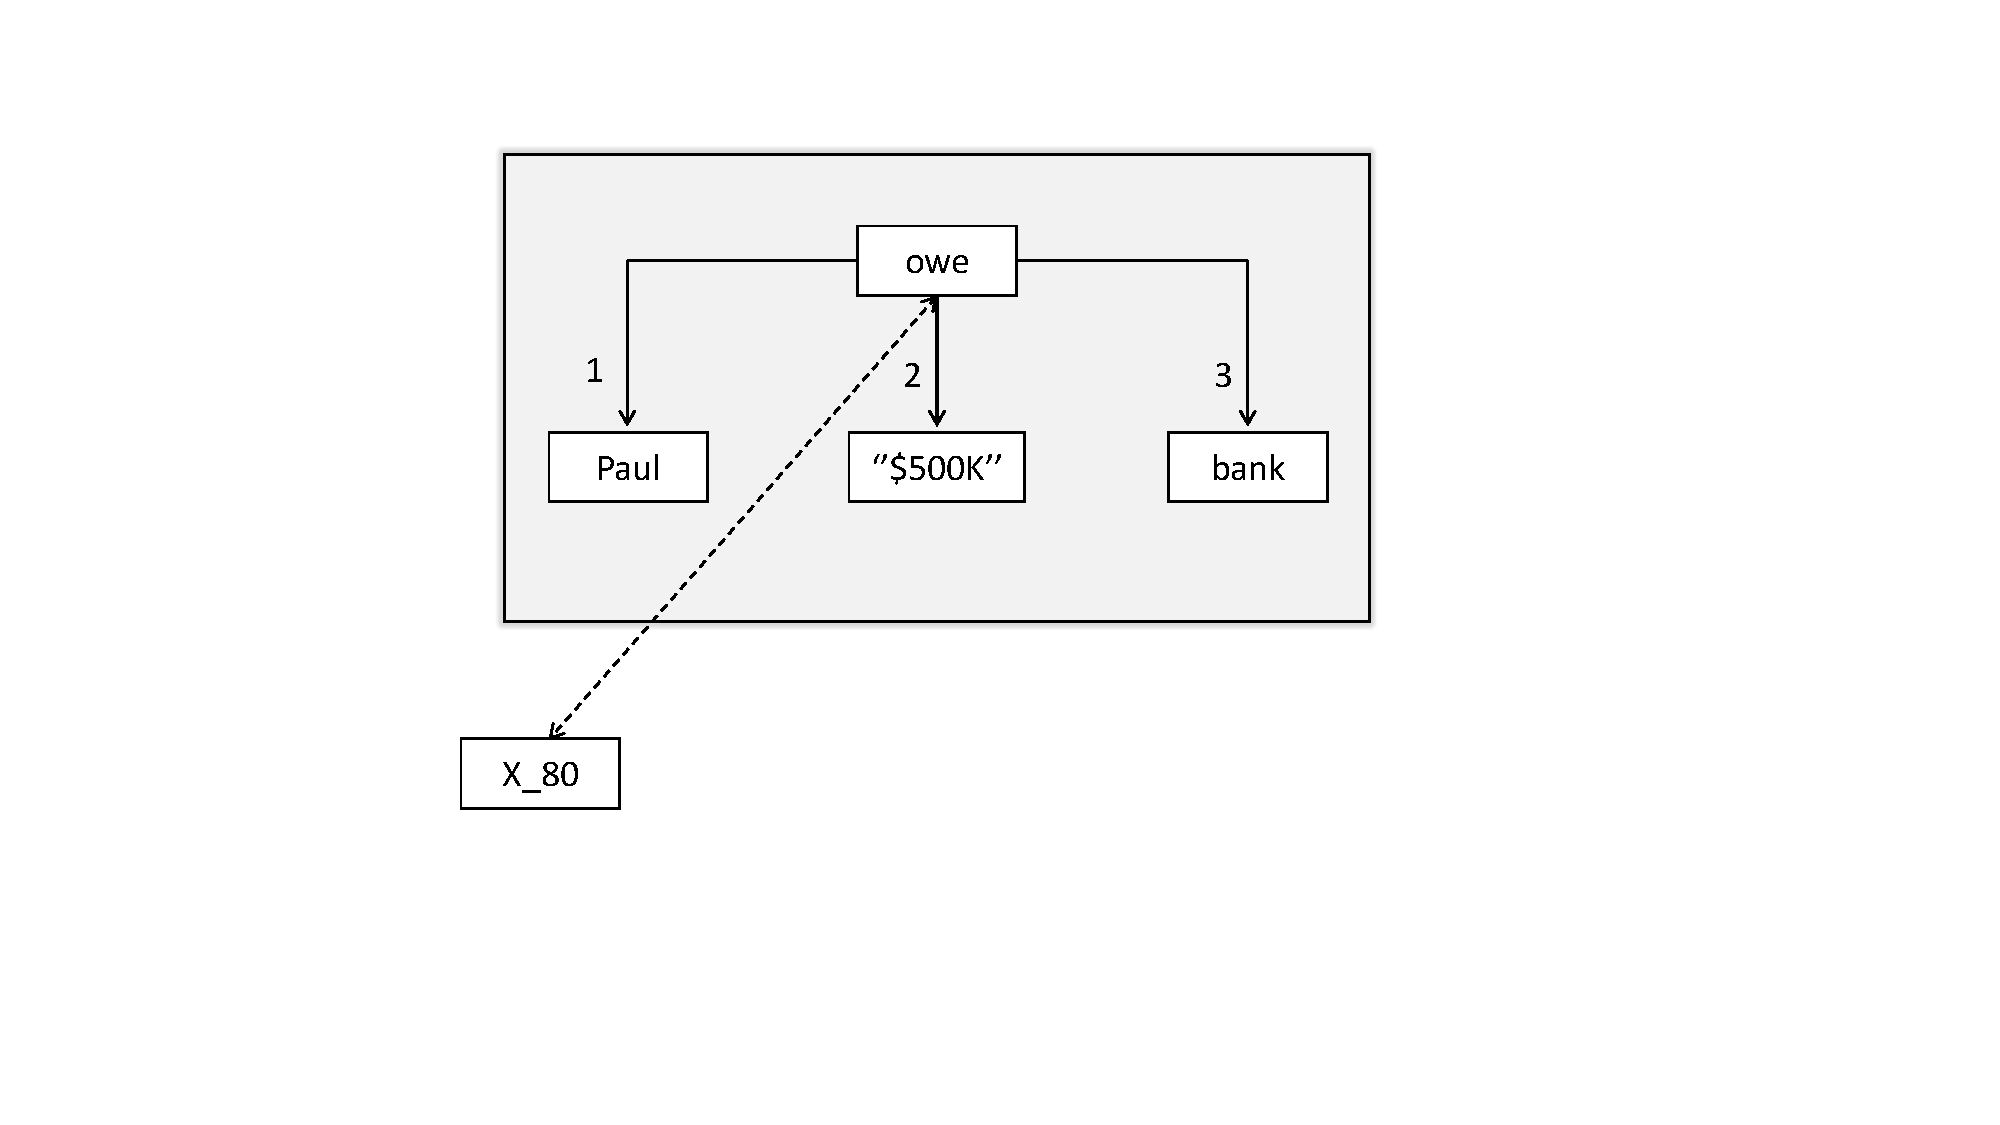
\includegraphics[width=1\textwidth, trim = {0cm 5cm 0cm 2cm},clip]{ch3/figs/root_standard.pdf}
	\vspace{-0.5cm}
	\caption{Application de \emph{root\_standard}}
	\label{fig:rootstand}
\end{figure}

\subsubsection{Application de la règle \emph{lex\_standard}}
La racine vide déclenchera l'application d'une règle de lexicalisation, c'est pourquoi GenDR fouillera dans le dictionnaire à la recherche des lexèmes représentant le sémantème \sem{owe}: \lstinline! owe { lex=owe lex=debt}!. GenDR peut ainsi lexicaliser la racine en choisissant \lex{debt}, ce qui entraînera l'application d'une fonction lexicale permettant de réaliser un verbe support sur la racine (ce qui satisfait la contrainte \texttt{dpos=V}). Il s'agit d'une lexicalisation complexe, donc nous renvoyons le lecteur à \cite{lambrey15,LambreyImplementationcollocationspour2017,lareau18} pour nous concentrer sur la lexicalisation simple effectuée grâce au lexème \lex{owe}.

\begin{figure}[htb]
	\centering
	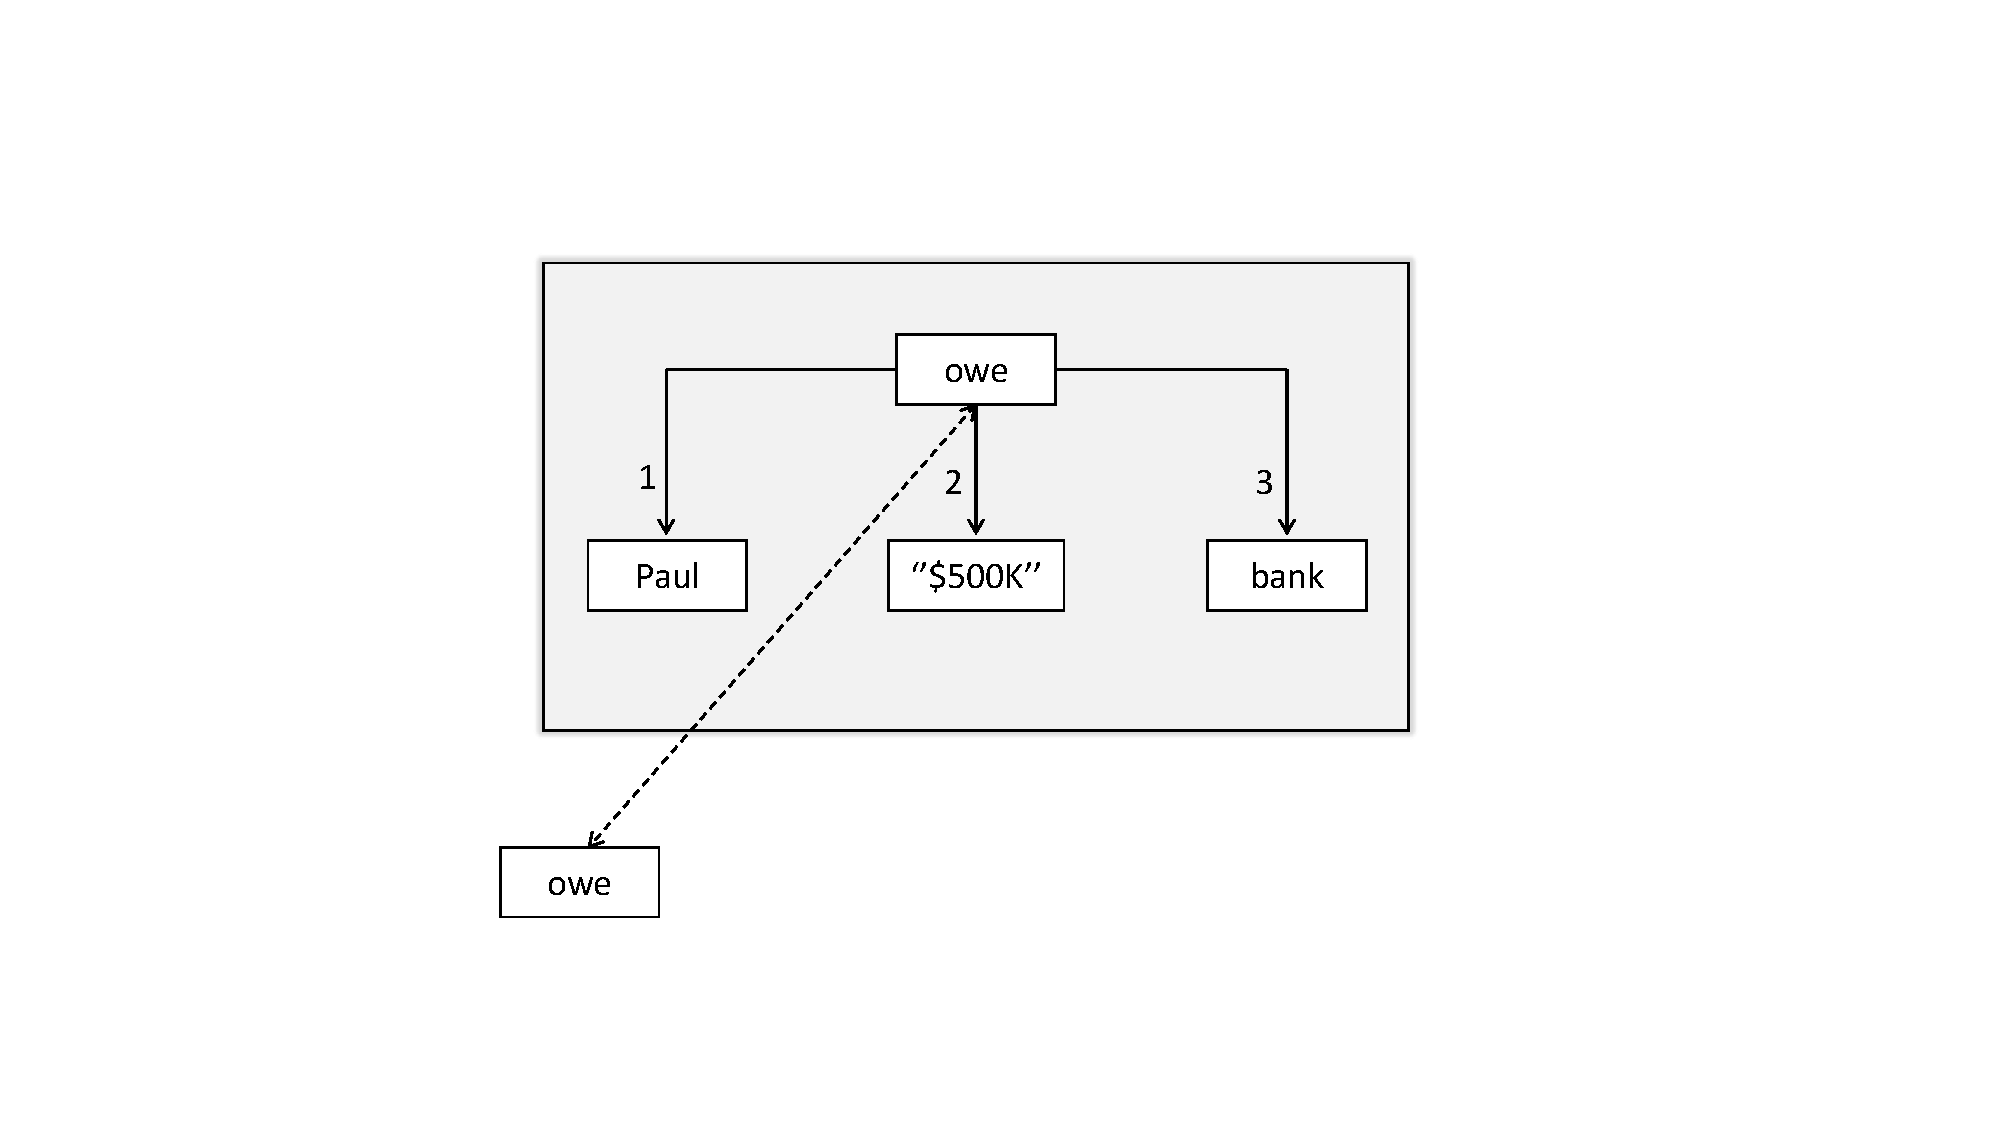
\includegraphics[width=1\textwidth, trim = {0cm 3cm 0cm 4cm},clip]{ch3/figs/lex_standard1.pdf}
		\vspace{-0.5cm}
	\caption{Application de \emph{lex\_standard}}
	\label{fig:lexstand1}
\end{figure}

\subsubsection{Application de la règle \emph{actant\_gp}}\label{sec:r-actantgp}
Une fois que la racine est pourvue d'un lexème, l'application de la règle \emph{actant\_gp} est déclenchée. Celle-ci traduit les relations sémantiques prédicat-argument de \sem{owe} en arcs syntaxiques profonds. La correspondance est confirmée par les informations sur la diathèse encodée dans le régime de la lexie \lex{owe}. Comme le prédicat lie trois actants sémantiques, alors la règle s'applique trois fois. Ensuite, les n\oe{}uds au bout des arcs syntaxiques seront contraints en fonction des restrictions prévues par le \ac{GP} de \lex{owe}. Ce mécanisme assure la grammaticalité de la construction de l'arbre. Pour cet exemple, le \ac{GP} de \lex{owe} permet à son deuxième actant syntaxique d'être soit un nom soit un nombre (la figure~\ref{fig:lexicon} montre le régime du verbe).

\begin{figure}[htb]
	\centering
	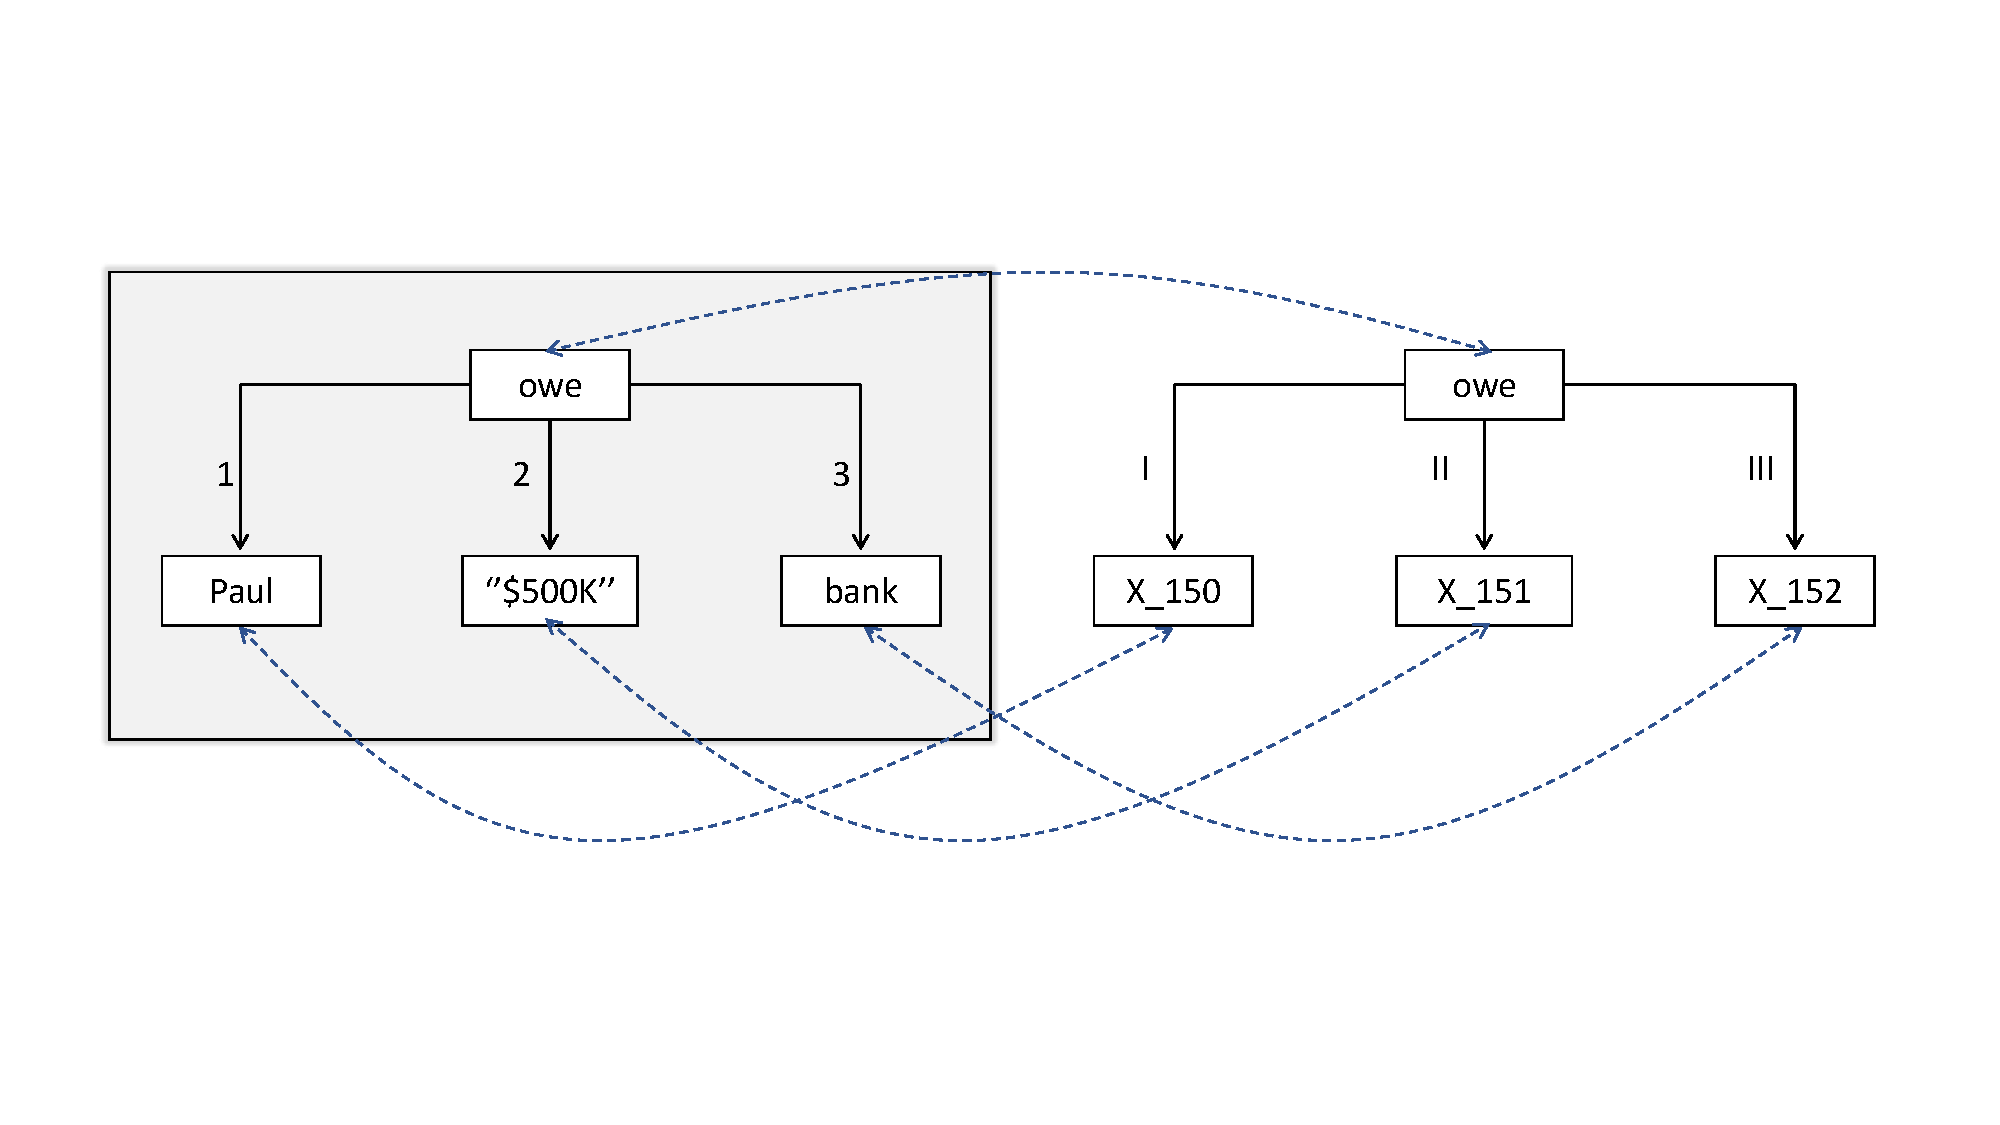
\includegraphics[width=1\textwidth, trim = {0cm 4.5cm 0cm 4cm},clip]{ch3/figs/application_actant_gp.pdf}
	\caption{Application de \emph{actant\_gp}}
	\label{fig:actantgp}
\end{figure}

\subsubsection{Application des règles \emph{lex\_class} et \emph{lex\_standard}}

L'étape précédente a généré des arcs contraints en partance de la racine. Les n\oe{}uds de ces arcs devront donc être lexicalisés afin de poursuivre la construction de l'arbre. GenDR appliquera deux règles de lexicalisation pour réaliser les lexèmes correspondant à \sem{Paul}, \sem{bank} et \sem{\$500}. D'abord, la règle \emph{lex\_class} sera utilisée puisque \sem{Paul} et \sem{\$500} affichent, respectivement, les traits \texttt{class=proper\_noun} et \texttt{class=amount} dans l'input sémantique. Cette règle fait en sorte que GenDR passe directement au \emph{lexicon}, puisque les sens ne sont pas décrits dans le \emph{semanticon}. L'étiquette du n\oe{}ud sémantique est directement copiée en syntaxe puis GenDR s'assure finalement que les traits de \lex{Paul} et \lex{\$500} respectent les contraintes des n\oe{}uds générés par la règle précédente. Ensuite, la règle \emph{lex\_standard} s'applique pour lexicaliser \sem{bank}.

\begin{figure}[htb]
	\centering
	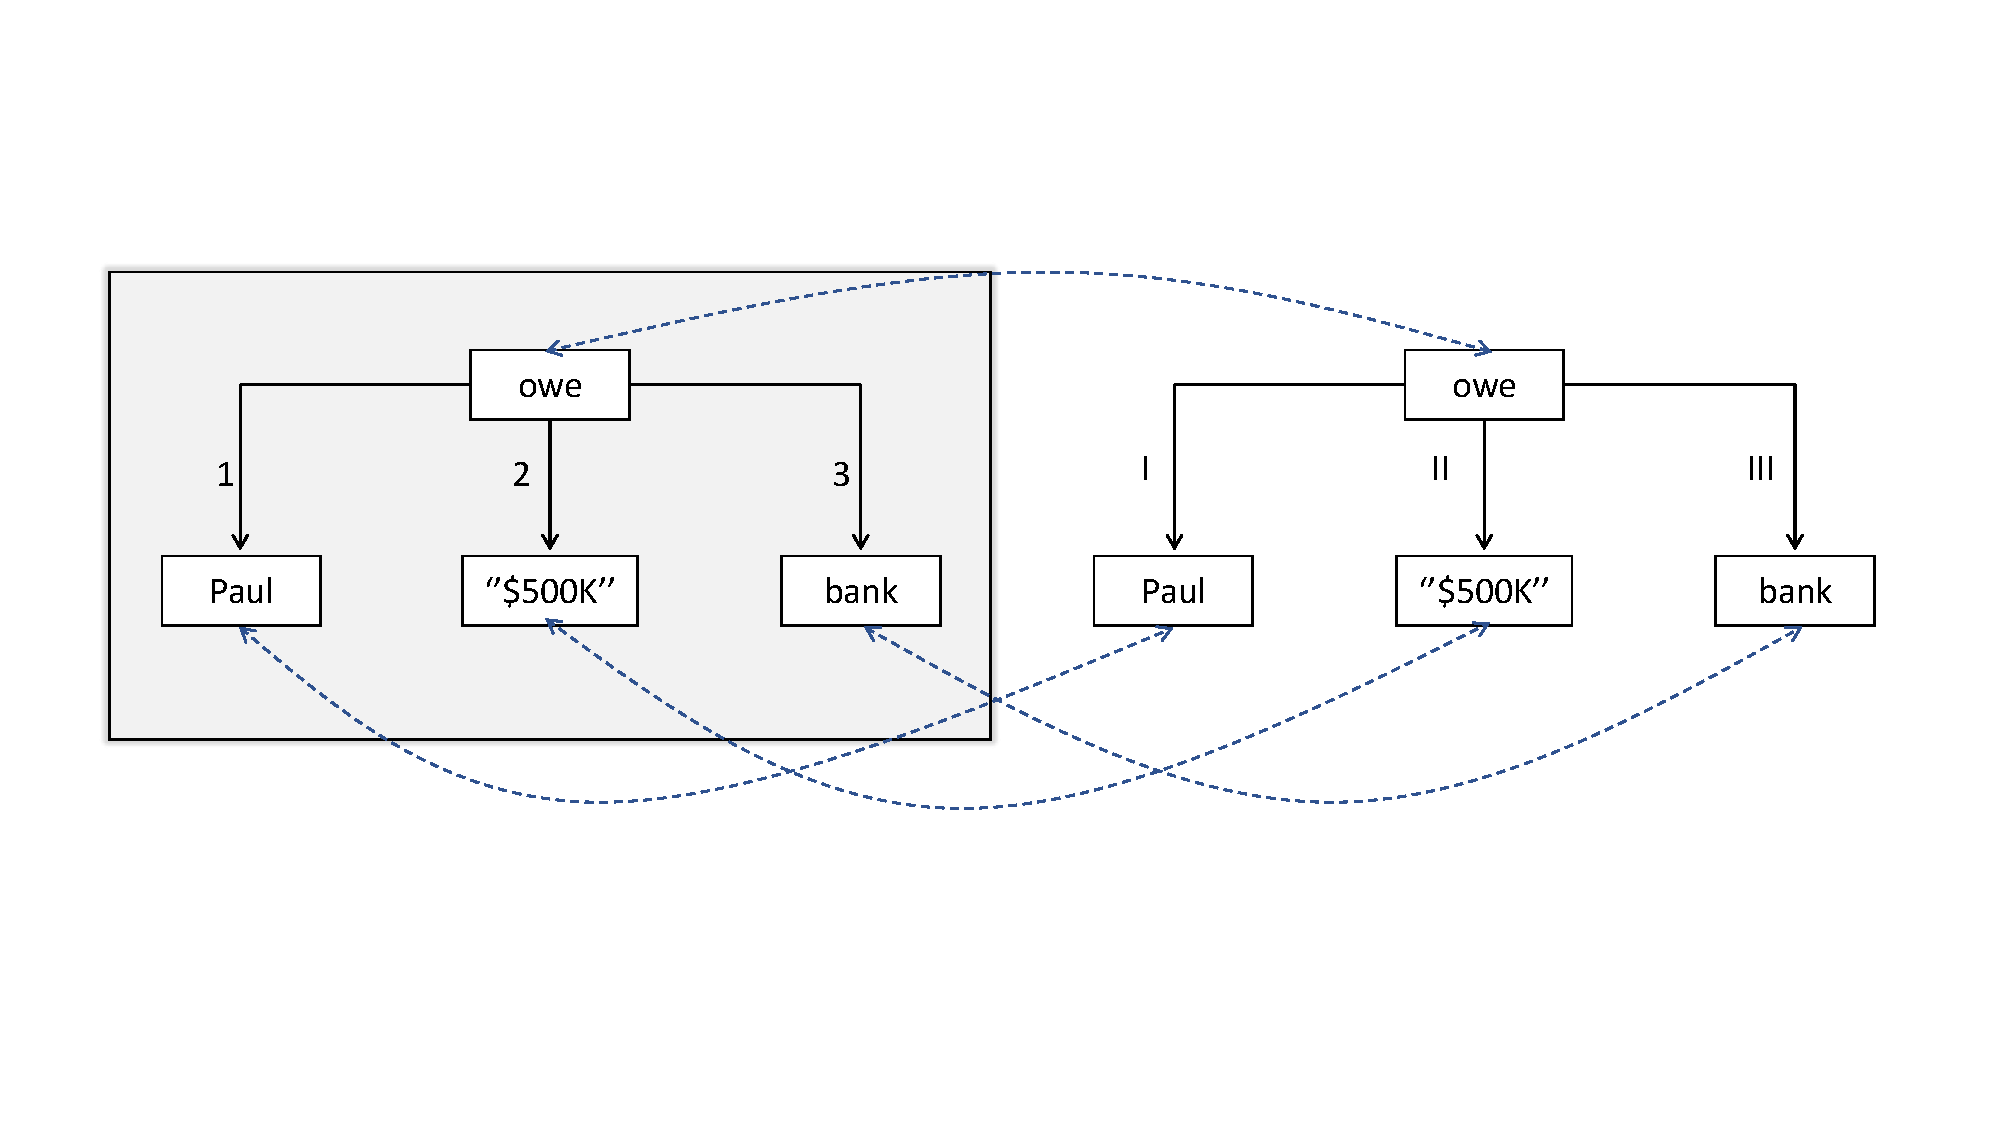
\includegraphics[width=1\textwidth, trim = {0cm 4.5cm 0cm 4cm},clip]{ch3/figs/lexical_2.pdf}
	\caption{Application des règles de lexicalisation}
	\label{fig:lexstand2}
\end{figure}

\subsection{Arborisation et lexicalisation de surface}

\subsubsection{Application des règles de lexicalisation de surface}

On récupère les lexicalisations de surface de chacune des unités lexicales avec les règles \emph{lex\_class} (qui s'occupe des lexèmes comme \lex{Paul}) et \emph{lex\_lu}. Il y en a deux, car il faut une règle spécifique pour les lexèmes appertenant à des classes puisque leurs traits de surface ne sont pas encodé dans leurs entrées lexicale, mais dans la classe qui leur est assignée.

\begin{figure}[htb]
	\centering
	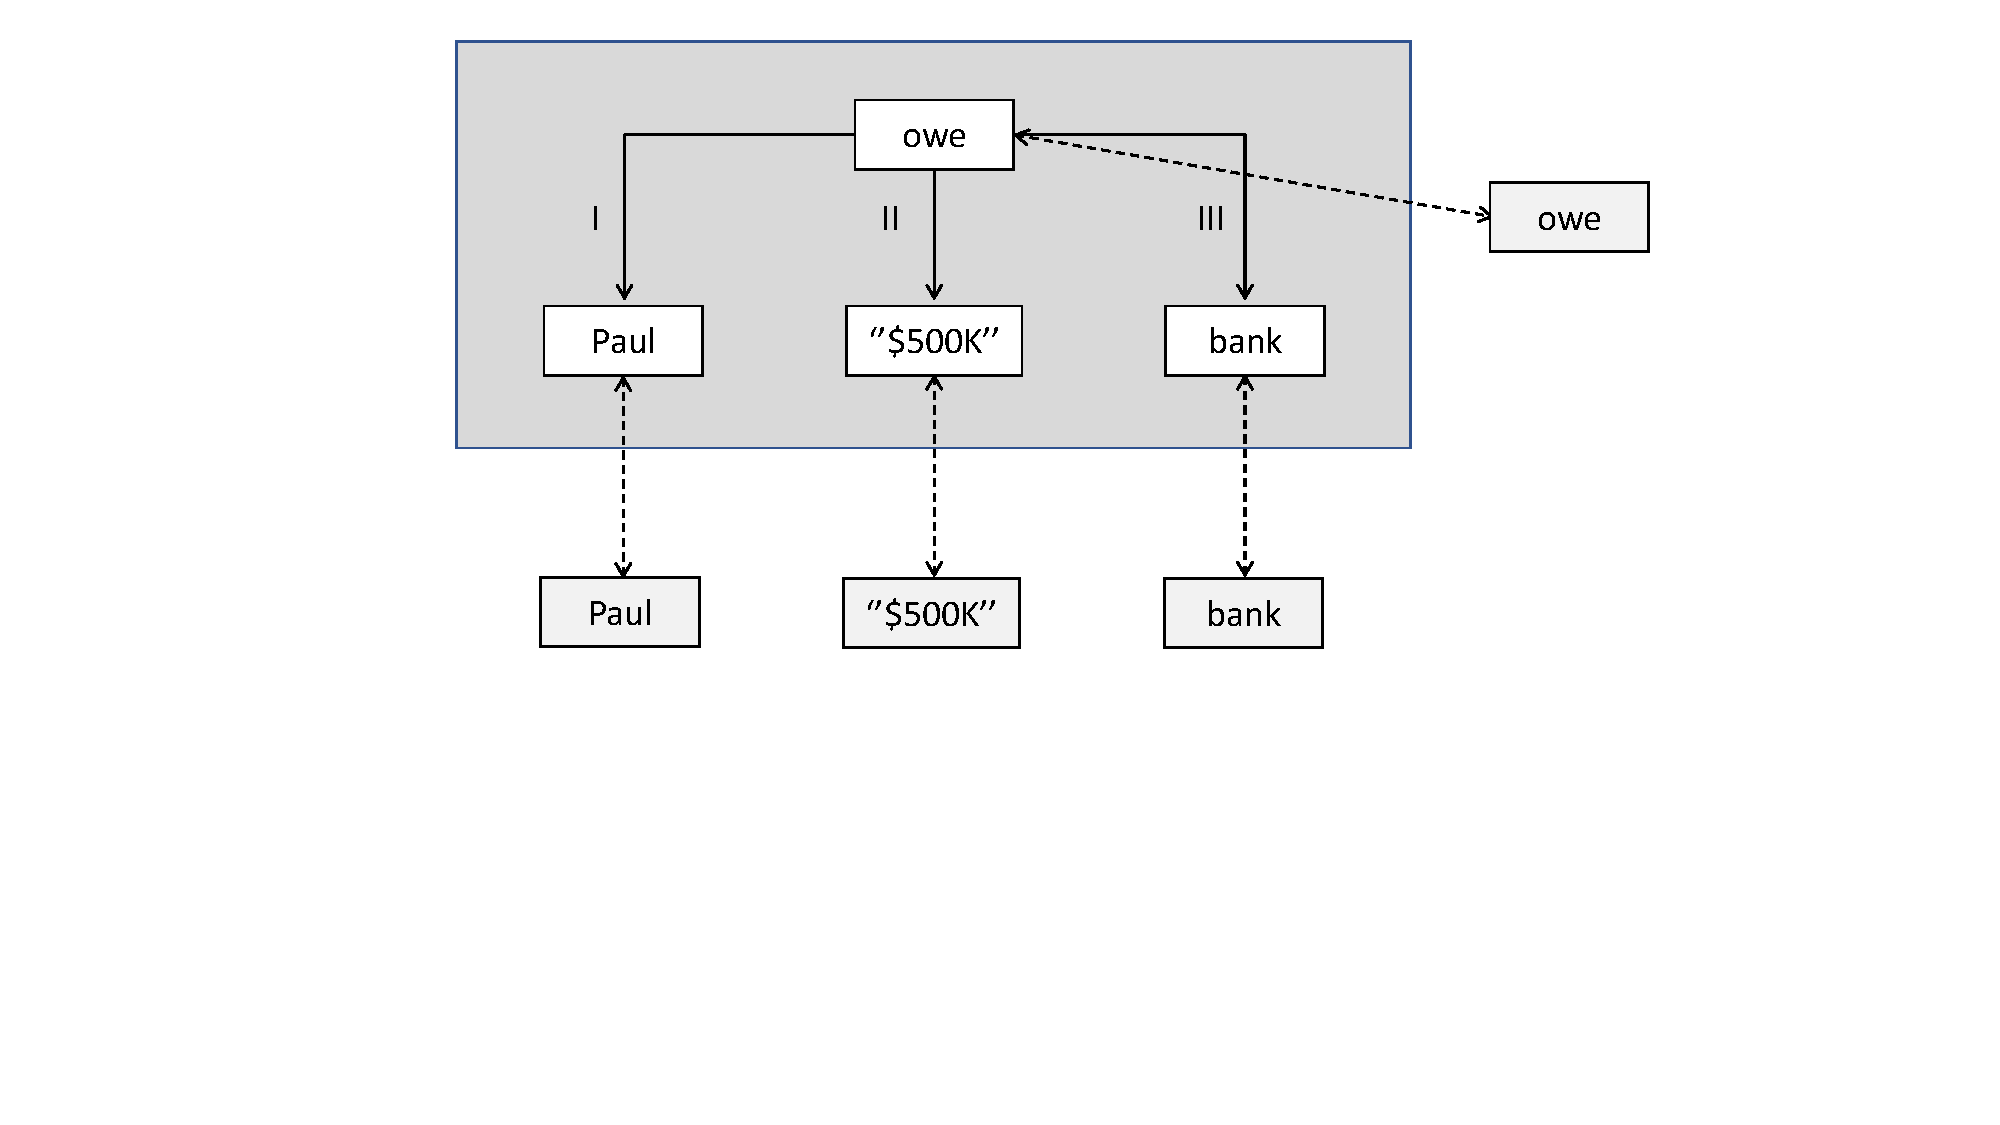
\includegraphics[width=1\textwidth, trim = {0cm 8cm 0cm 0.5cm},clip]{ch3/figs/lex_surf_gendr.pdf}
	\caption{Application des règles de lexicalisation de surface}
	\label{fig:lexsurf}
\end{figure}

\subsubsection{Application des règles actancielles de surface}
Ces règles remplacent les étiquettes des branches de l'arbre profond (I, II, III,...) par des étiquettes de surface (sujet, objet direct, objet indirect,...). Elles sont encodées dans le \ac{GP} du gouverneur de cette manière: \lstinline|gp = { I = { dpos = N \textbf{rel = subjective} } }|. Pour remplacer l'étiquette profonde par l'étiquette de surface de l'actant I, GenDR emploie la règle \emph{actant\_subj} qui récupère dans le \ac{GP} la valeur \texttt{subjective} et fait le remplacement nécessaire. Ensuite, il y a une règle qui s'occupe de la la relation objective directe (\emph{actant\_obj}). Celle-ci fonctionne de la même manière que la règle subjectale sauf qu'elle récupère la valeur de l'actant II et réalisera la valeur \texttt{dir\_objective}. 

Finalement, les relations indirectes/obliques sont à part car elles nécessitent la réalisation de n\oe{}uds intermédiaires en surface. C'est la règle \emph{actant\_prep} qui se charge de créer un n\oe{}ud intermédiaire en syntaxe de surface permettant d'accueillir le lexème fonctionnel nécessaire à la bonne formation de la phrase. La préposition est directement encodée dans le \ac{GP} du verbe, de cette manière: \lstinline! gp = {III = { dpos = N  rel = indir_objective  prep = to} }!.

\subsubsection{Application de la règle des déterminants}

La règle \emph{det\_def} ajoute les déterminants aux lexèmes en fonction de leur définitude. Parmi les règles que nous avons présentées, c'est la seule règle de GenDR qui est propre à l'anglais. Dans l'exemple présent, elle lexicalise \lex{the} puisque l'unité sémantique \sem{bank} était marquée par le trait défini dans la structure d'input.

La figure~\ref{fig:syntsurf} démontre l'application des règles actancielles et de la règle des déterminants.

\begin{figure}[htb]
	\centering
	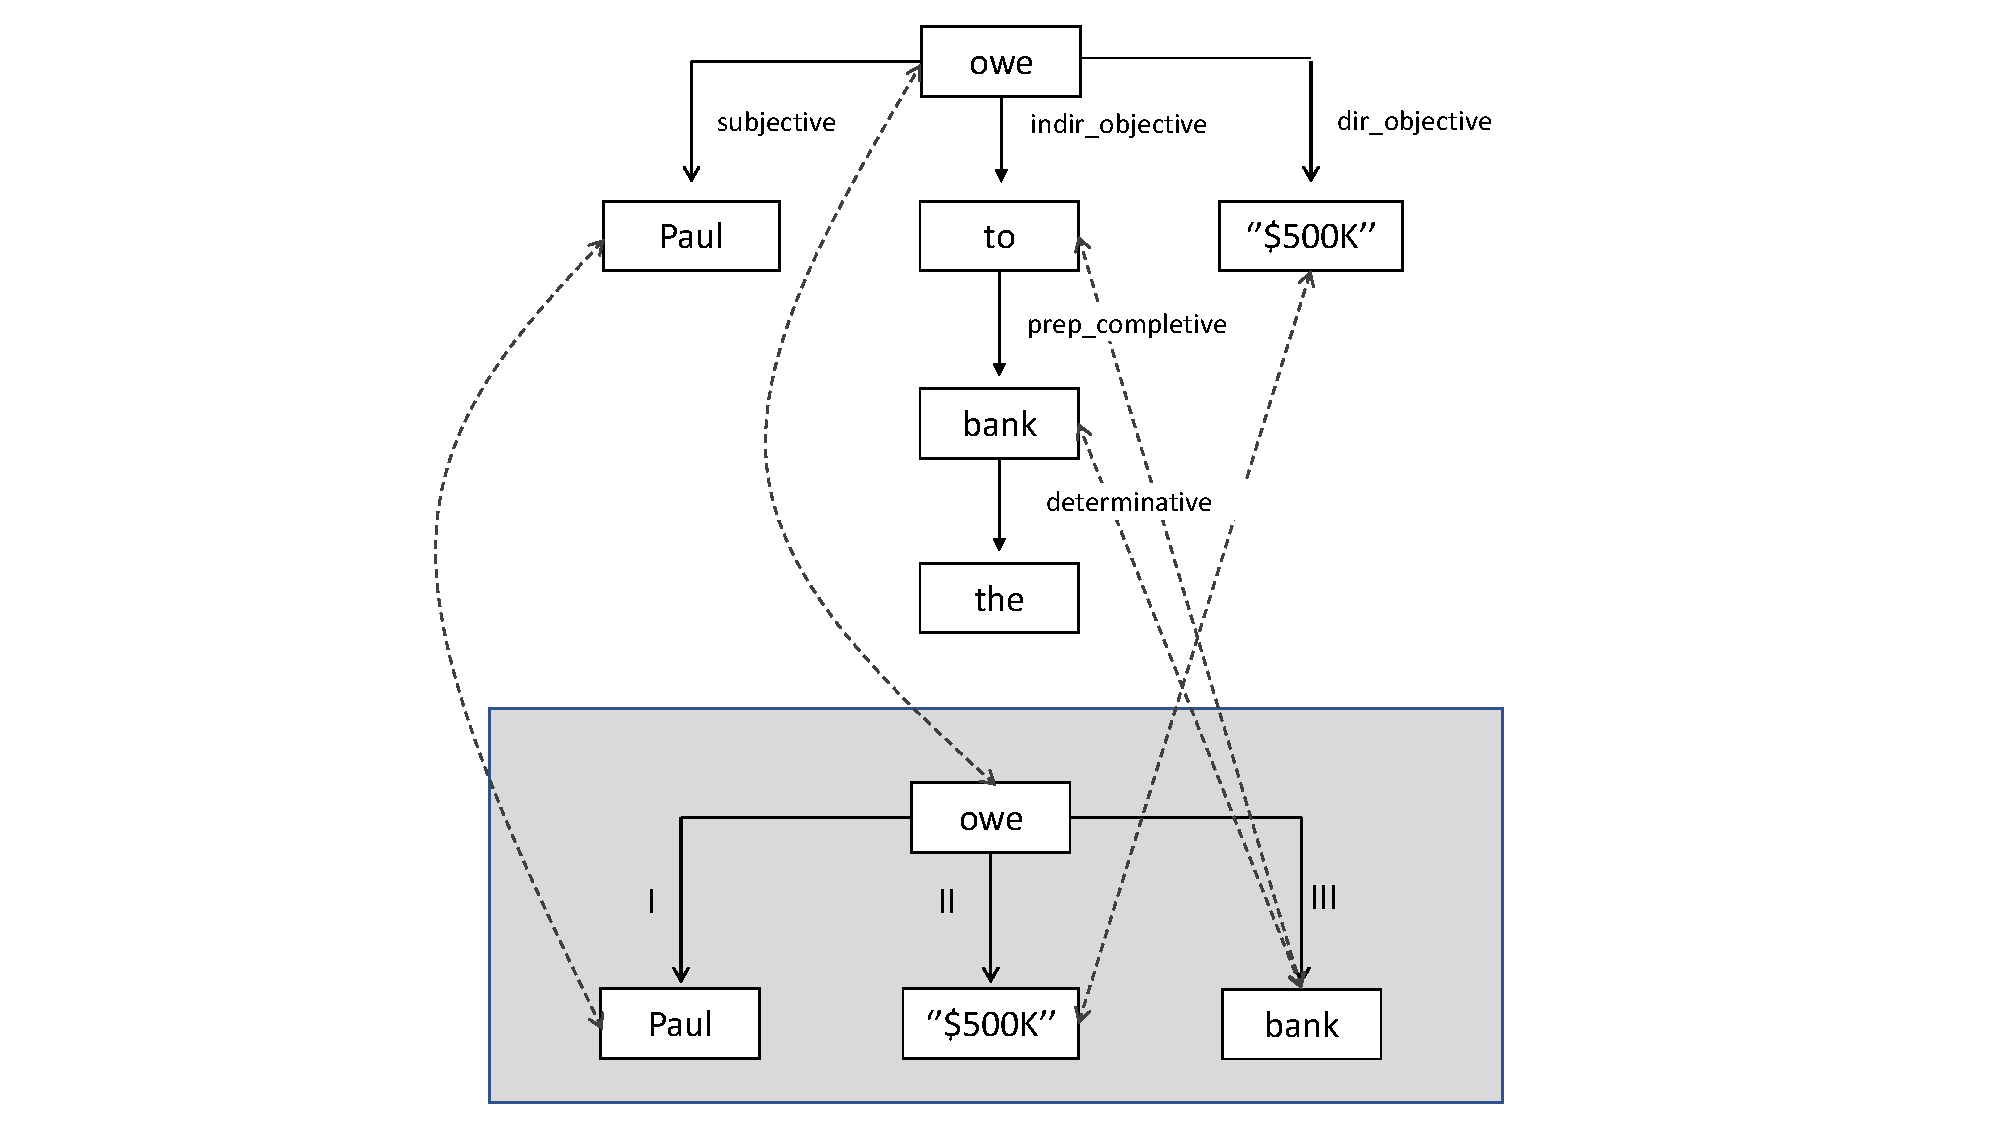
\includegraphics[width=1\textwidth, trim = {0cm 0cm 0cm 0cm},clip]{ch3/figs/final_surf_gendr.pdf}
	\caption{Application des règles actancielles de surface et des déterminants}
	\label{fig:syntsurf}
\end{figure}

%%%%%%%%%%%%%%%%%%%%%%%%%%%%%%%%%%%%%%%%%%%%%%%%
% --------- P R O B L É M A T I Q U E ---------
%%%%%%%%%%%%%%%%%%%%%%%%%%%%%%%%%%%%%%%%%%%%%%%%

\section{Problématique}\label{sec:problema}

L'exemple (section \ref{sec:exemple}) que nous venons d'illustrer démontre que GenDR modélise bien les phénomènes linguistiques profonds. Toutefois, le dictionnaire lexical de ce système ne couvre que les 1\,500 lexies les plus fréquentes (en anglais et en français). Parmi celles-ci, 500 sont des verbes, ce qui est non-négligeable, certes, mais il est clair que GenDR gagnerait en couverture s'il se dotait d'une ressource lexicale exhaustive décrivant les comportements des verbes. Nous pensons que de telles ressources sont nécessaires puisque les verbes contrôlent la structure de la plupart des énoncés et ils démontrent une grande variété quant à leur comportement syntaxique (qui est très imprévisible). Ainsi, en détenant les propriétés lexicales des verbes d'une langue donnée, on peut couvrir une grande partie des constructions syntaxiques possibles pour cette langue.

\begin{quote}
In particular, since verbs often convey the main idea of a sentence, such a resource must represent verb meanings. These require a particularly precise and well deffined representation that captures both their predicate-argument structure as well as their semantic content.
\end{quote}
\vspace{-\baselineskip}
\hfill
\cite{SchulerVerbnetBroadcoverageComprehensive2005}

Nous sommes en accord avec cette déclaration et nous ne sommes pas les seuls:  \cite{Korhonenlargesubcategorizationlexicon2006} suggèrent aussi que la modélisation informatique des langues naturelles passe par la création de dictionnaire renfermant les propriétés syntaxiques des verbes. Notre objectif est d'intégrer au réalisateur profond GenDR un dictionnaire de cadre syntaxique des verbes de la langue anglaise. De plus, comme GenDR se veut multilingue, si l'expérience fonctionne bien, l'objectif serait d'acquérir d'autres ressources lexicales similaires dans d'autres langues afin d'exploiter le réalisateur au maximum de sa capacité.

\section{Patrons de régime}\label{sec:gp}

Ce que plusieurs appellent des \scare{comportements syntaxiques} sont encodés dans des patrons de régime en TST. D'abord, il faut préciser que ce qu'on appelle \ac{GP} se nomme de différentes manières selon le cadre théorique utilisé: cadre valenciel, valence, cadre de sous-catégorisation, cadre syntaxique ou schéma de régime. Selon \cite{MilicevicSchemaregimepont2009}, les \acp{GP} décrivent les cooccurrences syntaxiques d'un lexème avec les actants qu'il régit. Par exemple, la relation entre un verbe et son sujet, ou bien la relation entre un nom et le complément qu'il sélectionne. Autrement dit, les \acp{GP} d'une lexie correspondent à l'ensemble des constructions syntaxiques que la lexie régit. On encode ces constructions syntaxiques dans un dictionnaire, car les \acp{GP} des lexèmes sont généralement imprévisibles. En effet, on ne peut pas prédire le nombre d'actants qu'un prédicat gouverne, ou bien les prépositions qu'il régit. En ce sens, même des verbes sémantiquement proches ne possèderont pas nécessairement les mêmes constructions syntaxiques, ce qui est illustré par \cite{MilicevicSchemaregimepont2009}: \form{on se souvient de $X$}, mais \form{on se rappelle $X$}.

\begin{quote}
Comme le choix lexical détermine le choix des constructions syntaxiques possibles (la lexie sélectionnée \og amène\fg\ avec elle son régime) et vice-versa (le choix d’une structure impose certains choix lexicaux), on peut dire que c’est le schéma de régime qui, au sein d’un [modèle Sens-Texte], fait le pont entre le lexique et la grammaire.
\end{quote}
\vspace{-\baselineskip}
\hfill
\cite[p.~105]{MilicevicSchemaregimepont2009}

À la section \ref{sec:semsynt}, nous avions parlé de l'interface sémantique-syntaxe et des règles de correspondance sémantiques qui font la transition \ac{RSem}--\ac{RSyntP}. Une partie du rôle du \ac{GP} est d'encoder les informations lexicales nécessaires pour que les règles de correspondances sémantiques génèrent des arbres profonds grammaticaux. 

En effet, les \acp{GP} contiennent l'information pertinente à l'arborisation (et à la lexicalisation) parce qu'ils renferment les données sur la diathèse d'un lexème. La diathèse, c'est le trait qui fait la correspondance entre les actants sémantiques d'une lexie et ses actants syntaxiques profonds. Elle est spécifiée dans les entrées lexicales d'un dictionnaire de cette manière : \lstinline|{1 = I, 2 = II, etc.}|. Dans ce scénario, le premier actant sémantique correspond au premier actant syntaxique et ainsi de suite (il s'agit d'une diathèse triviale), comme dans \form{Paul aime le ski}, où le sémantème \sem{aimer} et le lexème lex{aimer} placent leurs actants dans le même ordre. Le premier actant sémantique est \sem{Paul} et le second \sem{ski}, puis l'ordre entre ces actants est conservé en syntaxe profonde. Toutefois, si on lexicalise \sem{aimer} par le lexème \lex{plaire}, alors la diathèse est différente: \lstinline|{ 2 = I, 1 = II }|. Cela n'affecte en aucun cas le sens de l'énoncé: \sem{Le ski plaît à Paul}=\sem{Paul aime le ski}. Ensuite, au niveau du passage à la syntaxe de surface, le \ac{GP} encode aussi la réalisation des actants syntaxique en relation de surface où on passe d'une étiquette en chiffre romains à une étiquette superficielle: \lstinline|{ I = { rel = subjective } }|, l'actant \texttt{I} correspond au sujet.

De plus, le \ac{GP} encode les conditions dans lesquelles une structure syntaxique est exprimée. Par exemple, c'est dans le \ac{GP} qu'on précise que le troisième actant syntaxique doit être de telle partie du discours et qu'il sélectionne telle préposition. Ces conditions décrivent la combinatoire lexicale et syntaxique d'une lexie donnée. Par exemple, dans le dictionnaire de GenDR, cela est encodé ainsi: \lstinline|{ gp = {III = { dpos = N  rel = indir_objective  prep = to} } }|. Ainsi, grâce à ces restrictions, les règles de correspondances construiront des arbres de bonne formation.

Également, l'une des raisons qui nous a poussé à nous tourner vers une ressource lexicale verbale provient des limites du logicel MATE quant à l'encodage de multiples patrons de régime pour une même entrée. Par exemple, pour un verbe donné, on ne peut pas avoir deux parties du discours différentes compétitionnant pour la même position syntaxique. Autrement dit, si nous voulions exhaustivement représenter les comportements du verbe \lex{want}, il nous faudrait un \ac{GP} qui puisse tenir compte du fait que le second actant syntaxique de ce verbe peut avoir une \ac{DPOS} de type verbale ou nominale: \form{I want to eat} vs \form{I want a dog}. Cela nous était impossible à encoder dans MATE avec les paramètres que nous avions car le système ne nous laissait pas donner deux versions de l'actant syntaxique II de \lex{want}. Ce qui s'offrait à nous comme solution était de créer deux verbes \lex{want} qui encoderaient séparément ces comportements syntaxiques, ce qui n'était pas viable. Nous nous sommes alors tournés vers l'idée d'ajouter un dictionnaire supplémentaire à notre ressource, qui encoderait tous les régimes existants de l'anglais. Puis, nous n'aurions qu'à encoder l'identification des \ac{GP} dans les unités lexicales appropriées ce qui nous permettait de contourner le problème des \acp{GP} multiples.

Notre ancienne méthode restreignait conséquemment le nombre de réalisations possibles pour un verbe donné ou peuplait inutilement le dictionnaire d'entrées verbales quasi-identiques mais qui se distinguaient en fonction des régimes différents. 

En résumé, nous enrichissons considérablement le contenu lexical de notre dictionnaire en plus de trouver une solution au problème mentionné ci-haut. Pour trouver la bonne ressource, nous avons regardé les candidats qui s'offraient à nous, puis nous avons choisi celui qui correspondait le plus à nos besoins et qui pouvait s'intégrer le mieux à notre système. Le chapitre suivant est dédié à ces ressources lexicales, et nous décrirons celui que nous avons choisi, VerbNet.

